We now present the numerical results on stability for PF and EnKF, as well as the dependence of the exponential rates on the observation gap $g$ and the observation noise strength $\sigma$. In the following figures~\ref{fig:bpf-enkf-fixed-ocov--probing-nfs}-\ref{fig:bpf-enkf-fixed-ogap--probing-nfs}, in top row in each of the figures, the dots represent distance $D_\varepsilon(\pi_n(\mu_0), \pi_n(\mu_b))$ between the posterior distributions at time $t=ng$ with the initial distribution $\mu_0$ and $\mu_b$ mentioned in~\eqref{eq-3ic--probing-nfs} versus time for 10 realizations of the observational noise. We also plot the mean $\mathbb{E}[D_\varepsilon]$ averaged over these 10 observational realizations, and the best-fit curve~\eqref{eq:fit--probing-nfs} in the same figures. Rows 2 and 3 contain, respectively, the expectation value of scaled $l_2$ error $\mathbb{E}[e_n^2]$ and uncertainty $\mathbb{E}[s_n^2]$ defined in~\eqref{eq-error--probing-nfs} and \eqref{eq-var--probing-nfs} versus time. Row 4 contains scatter plot of RMSE, defined as the square root of the expected value of $e_n^2$, averaged over the 10 observational realizations, for the filter with biased initial distribution $\mu_b$ versus the mean $D_\varepsilon$ between posteriors from the biased and the unbiased initial distributions.

\subsection{Dependence on observation gap}
We first discuss the results of assimilation with both PF and EnKF for a fixed observation covariance $\sigma^2 = 0.4 I$ with varying observation gap. As shown in figure~\ref{fig:bpf-enkf-fixed-ocov--probing-nfs}, the mean $D_\varepsilon$ falls exponentially over time until reaching a stationary value for both the filters. Table~\ref{table:fixcov--probing-nfs} shows the values of the coefficients of the best-fit of mean $D_\varepsilon$ versus time, according to~\eqref{eq:fit--probing-nfs}, for different observation gaps $g$.




\begin{figure}[t!]
\centering
Particle filter $\qquad \qquad \qquad \qquad \qquad \qquad \qquad \qquad $ EnKF\\
    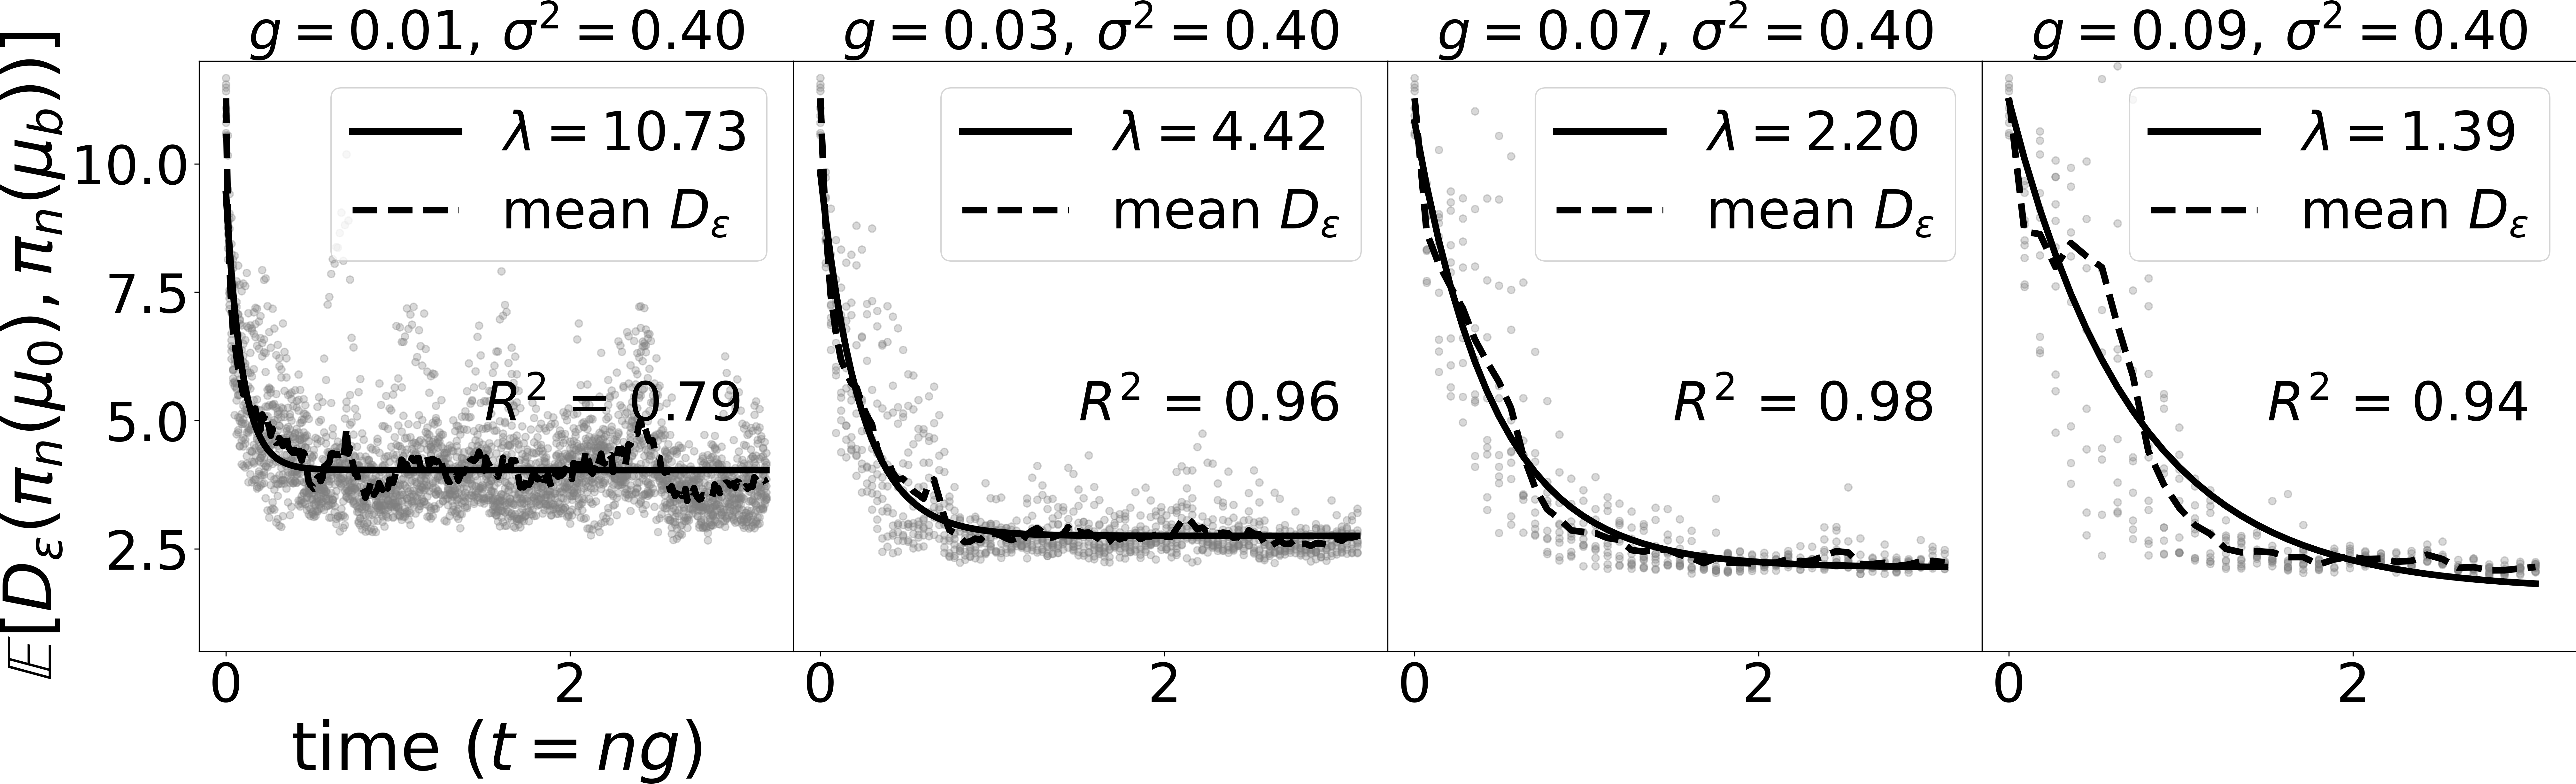
\includegraphics[width=0.48\textwidth]{probing-nfs/plots/plots-bpf-effect of obs gap-rate_obs_gap_all.png} $\ \ $
    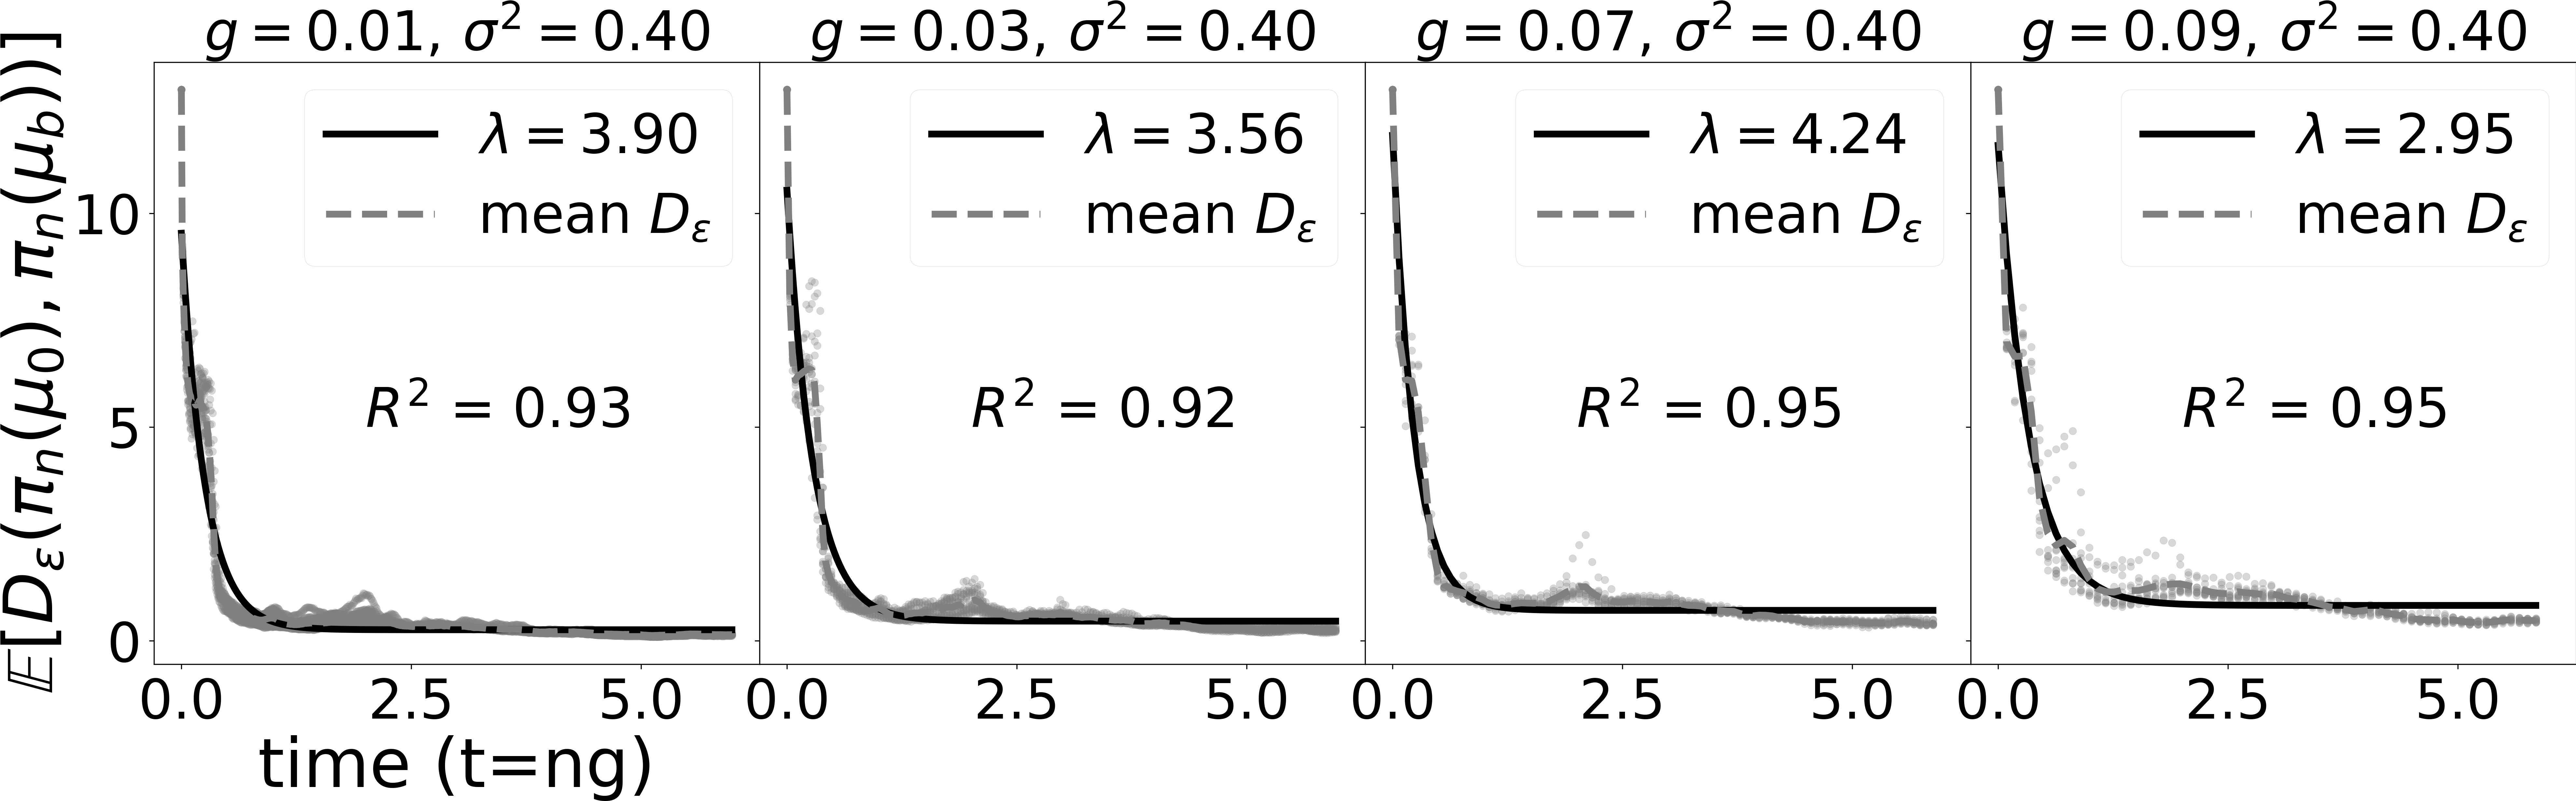
\includegraphics[width=0.48\textwidth]{probing-nfs/plots/plots-enkf-effect of ob gap-rate_all.png}\\
   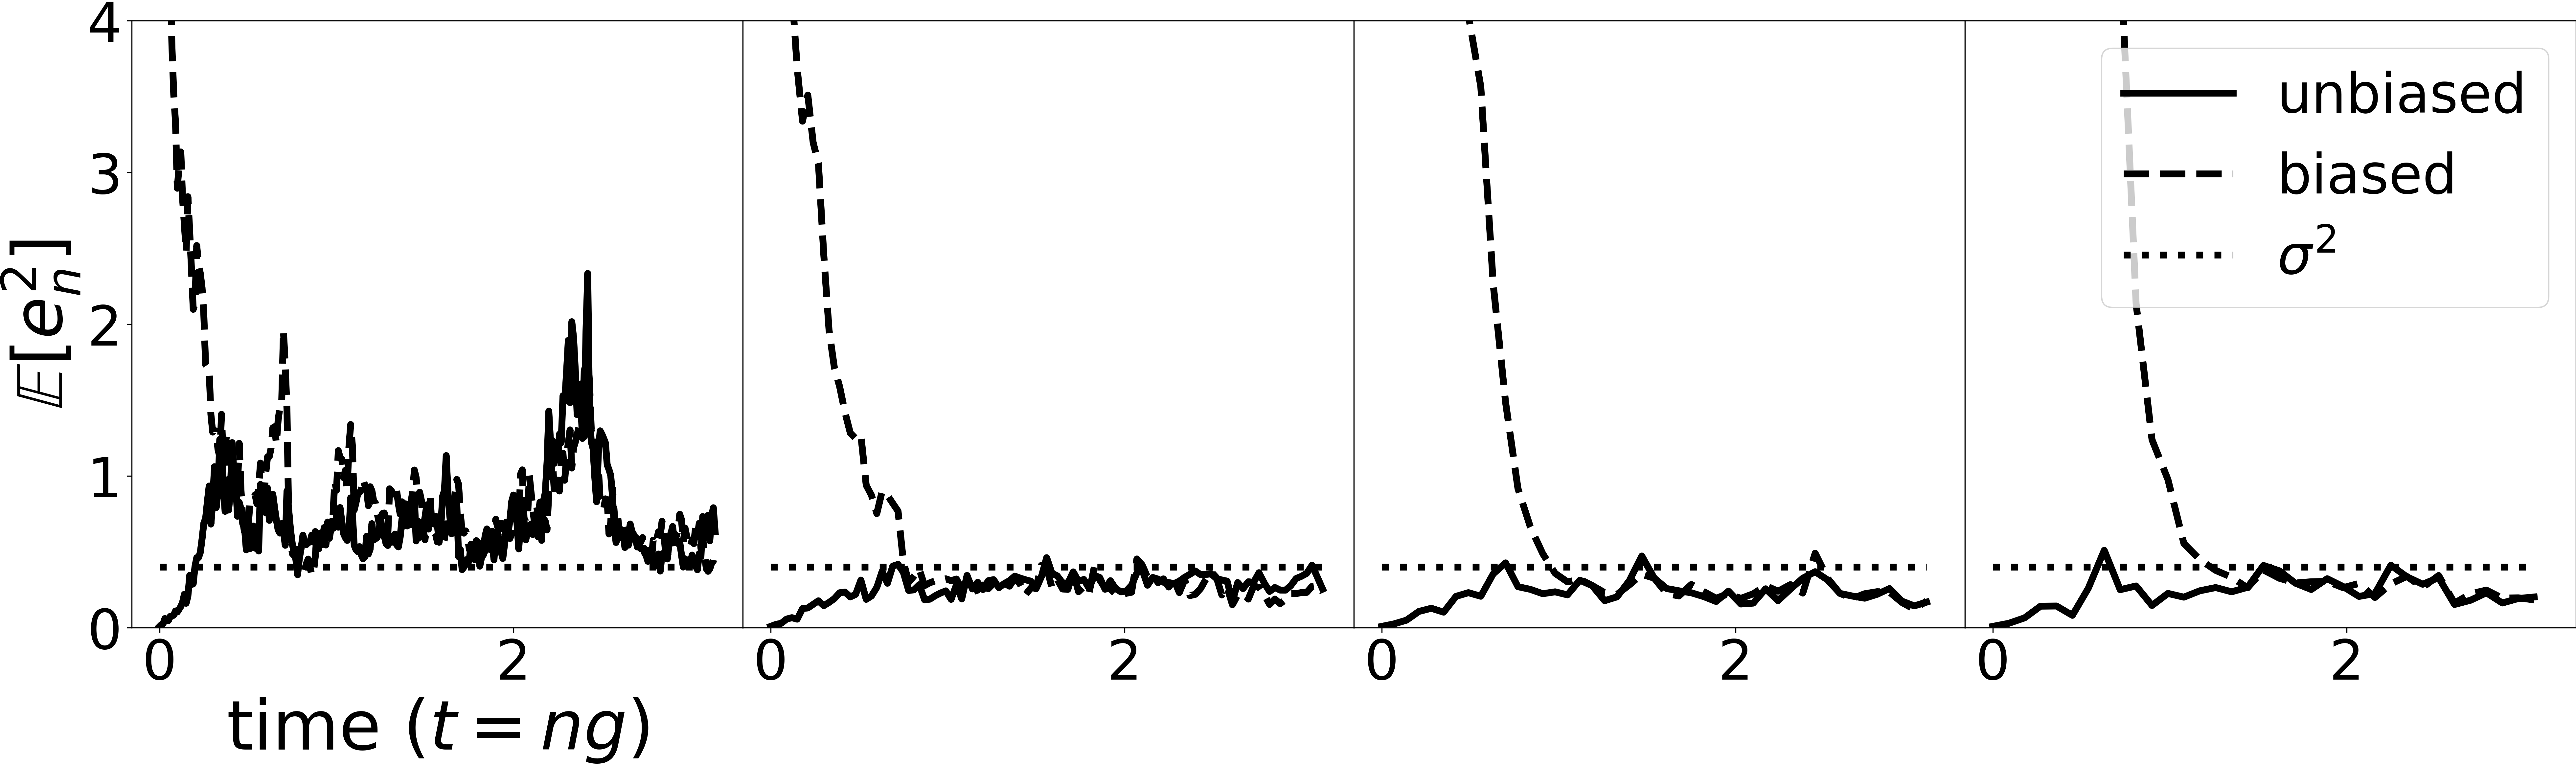
\includegraphics[width=0.48\columnwidth]{probing-nfs/plots/plots-bpf-effect of obs gap-l2_obs_gap_all.png} $\ \ $
    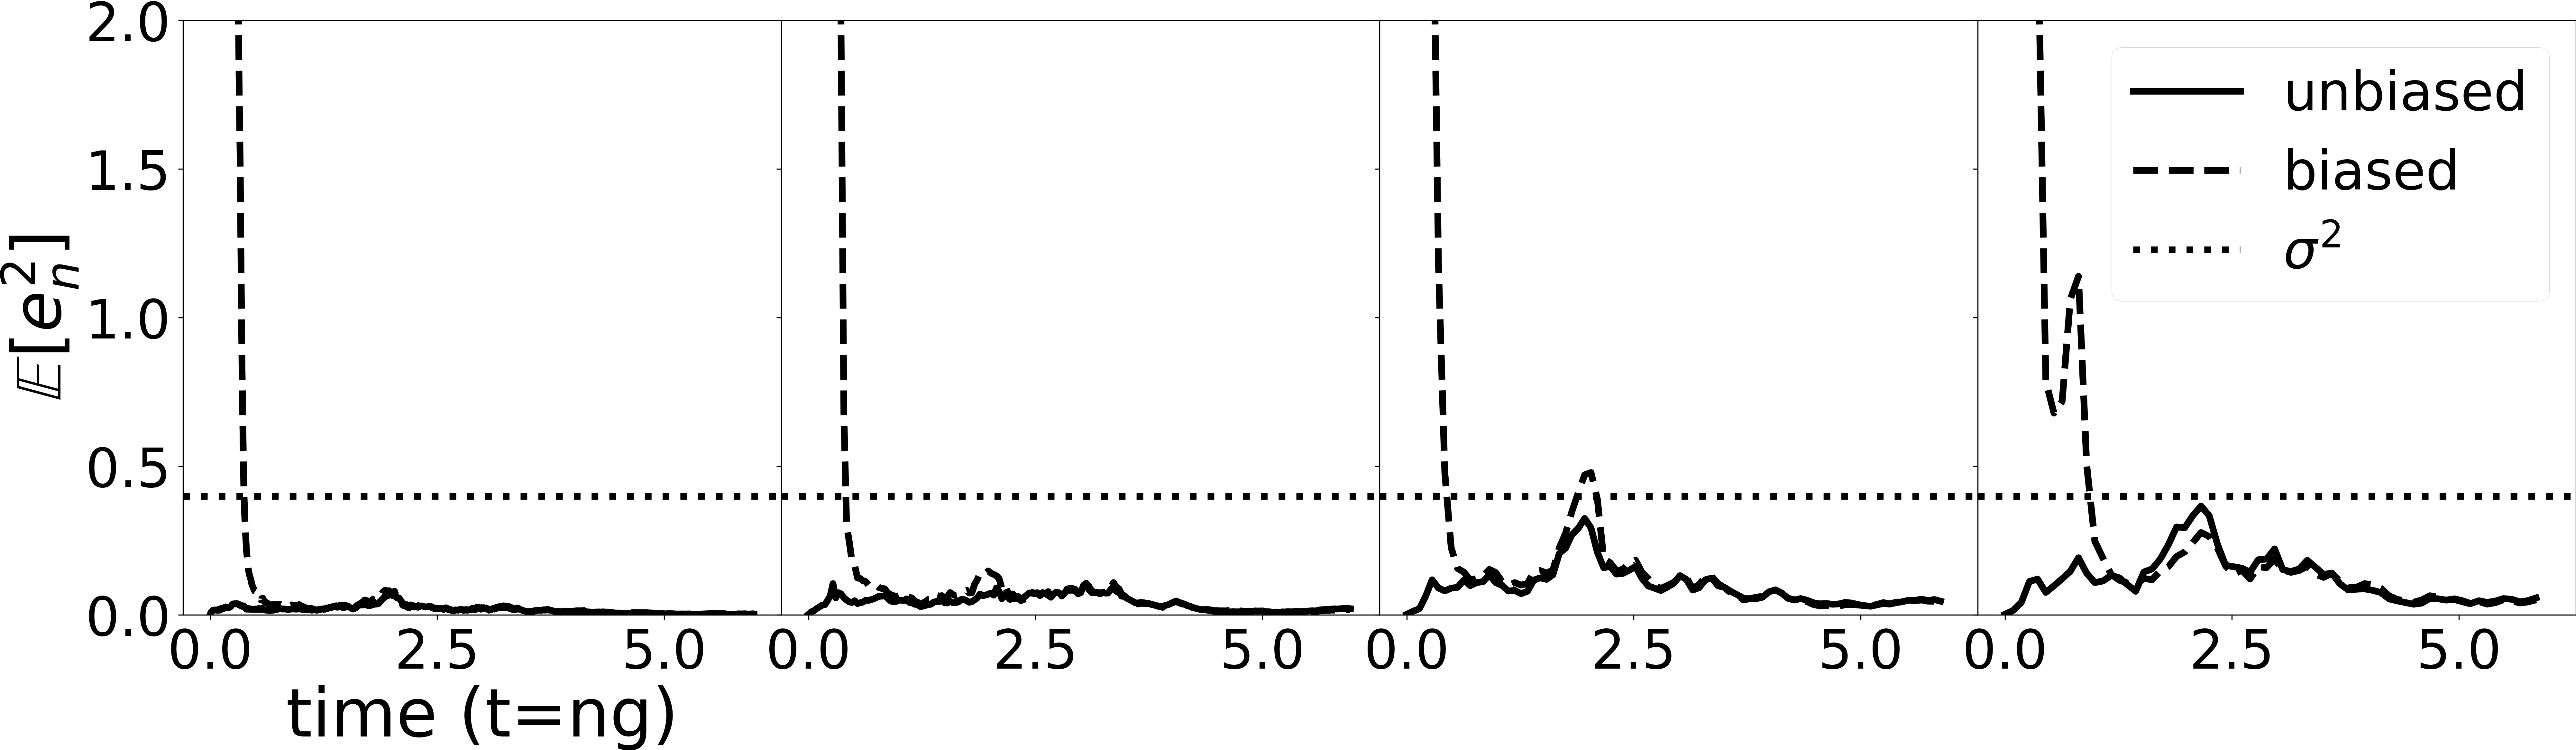
\includegraphics[width=0.48\textwidth]{probing-nfs/plots/plots-enkf-effect of ob gap-mean_l2error_all.png}\\
   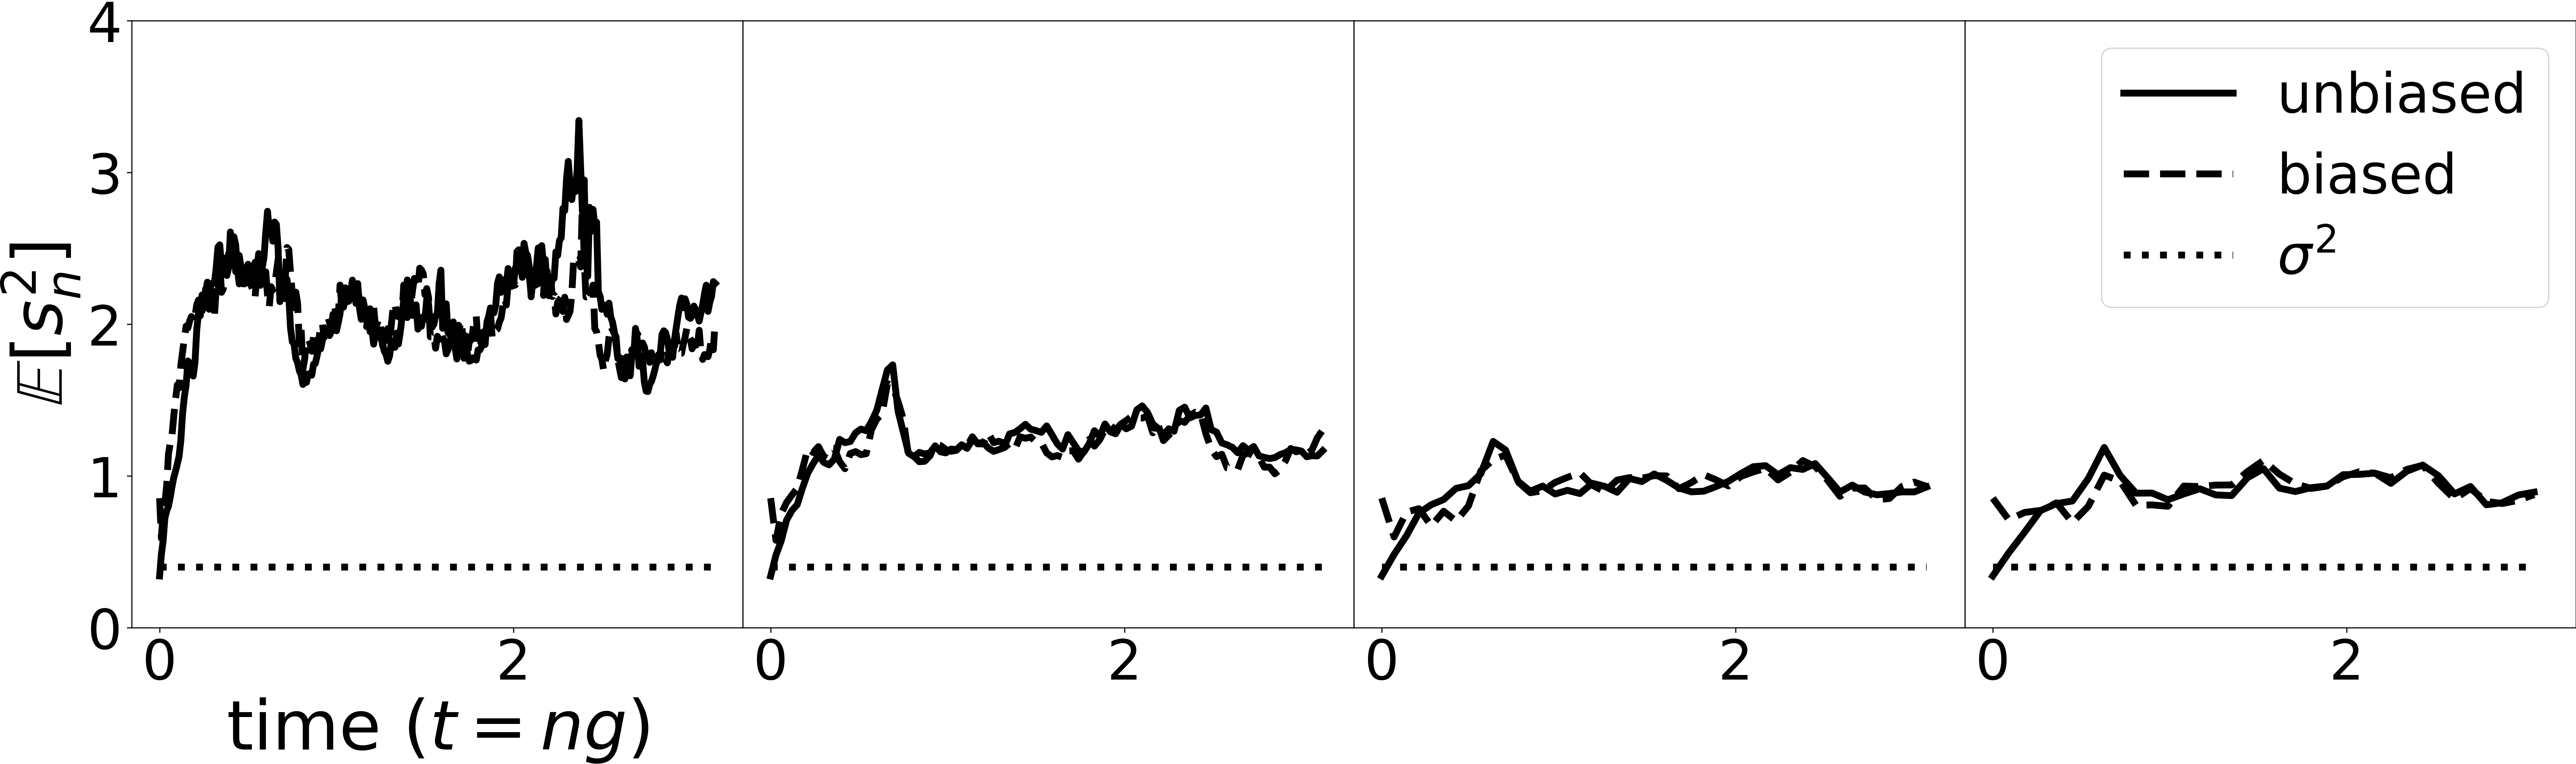
\includegraphics[width=0.48\columnwidth]{probing-nfs/plots/plots-bpf-effect of obs gap-trace_obs_gap_all.png} $\ \ $
    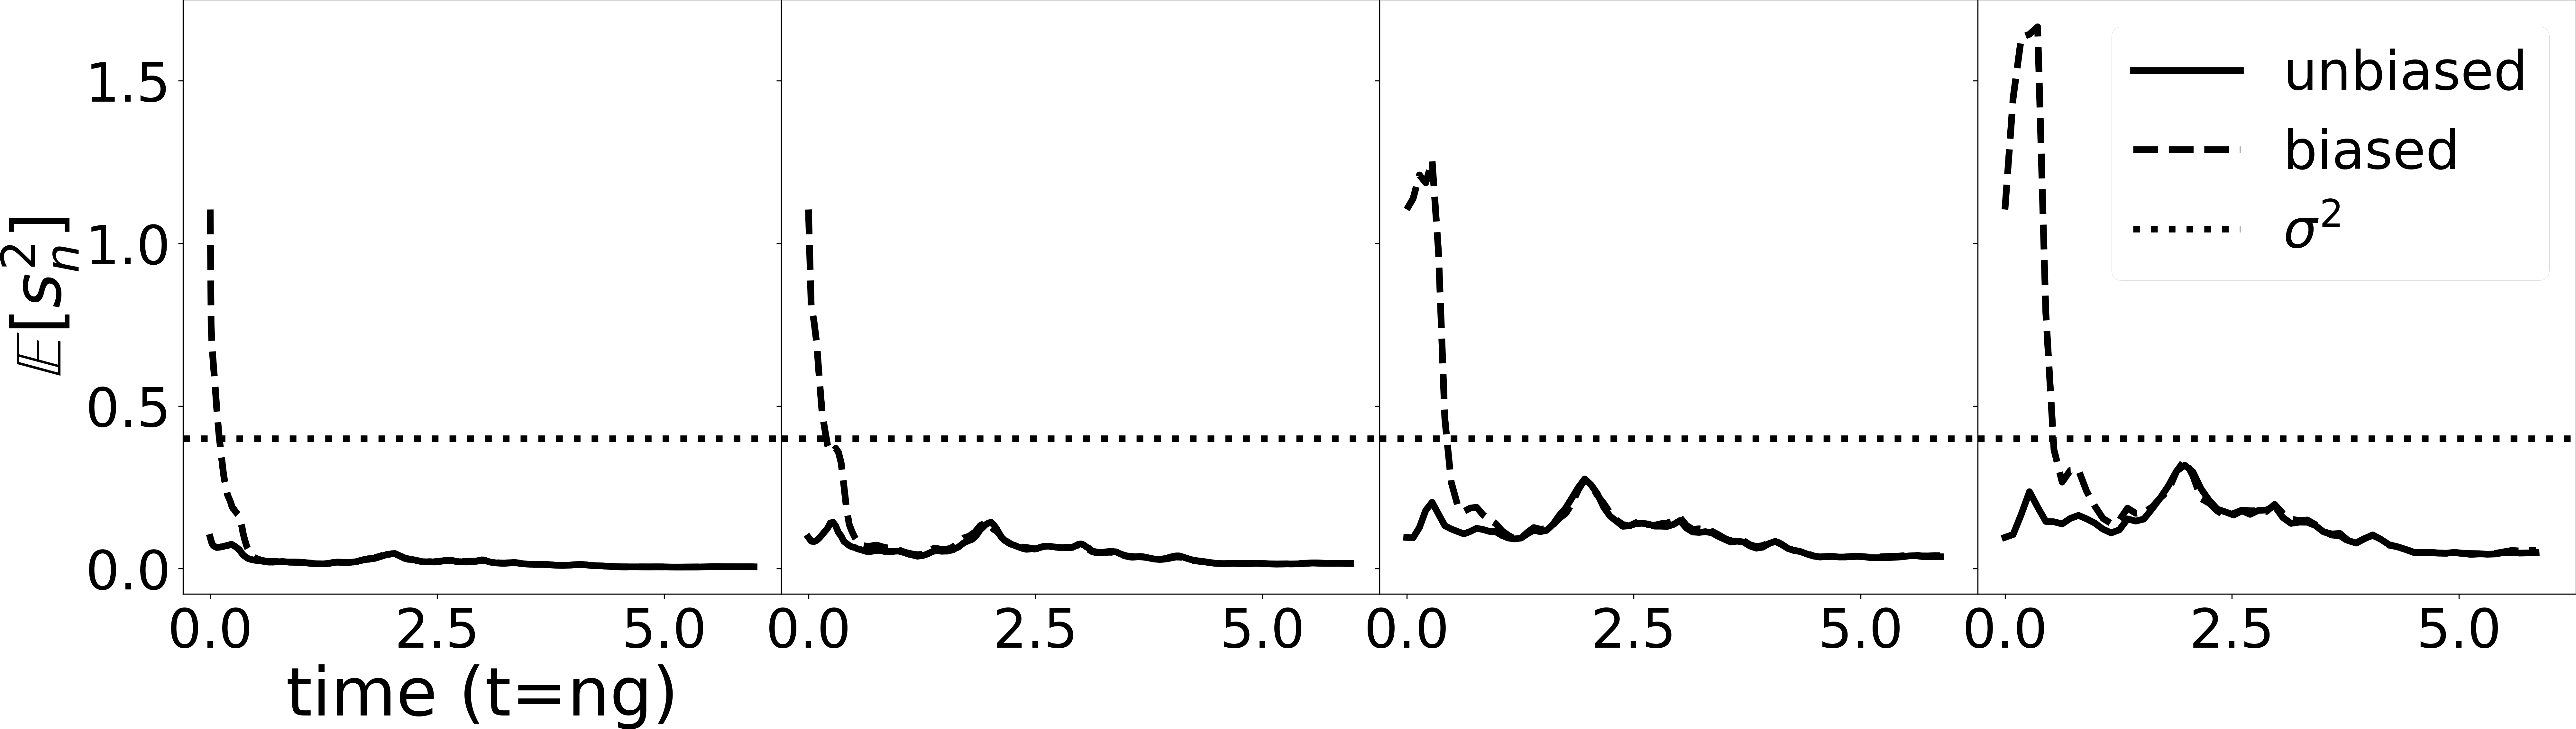
\includegraphics[width=0.48\textwidth]{probing-nfs/plots/plots-enkf-effect of ob gap-mean_trace_all.png}\\
   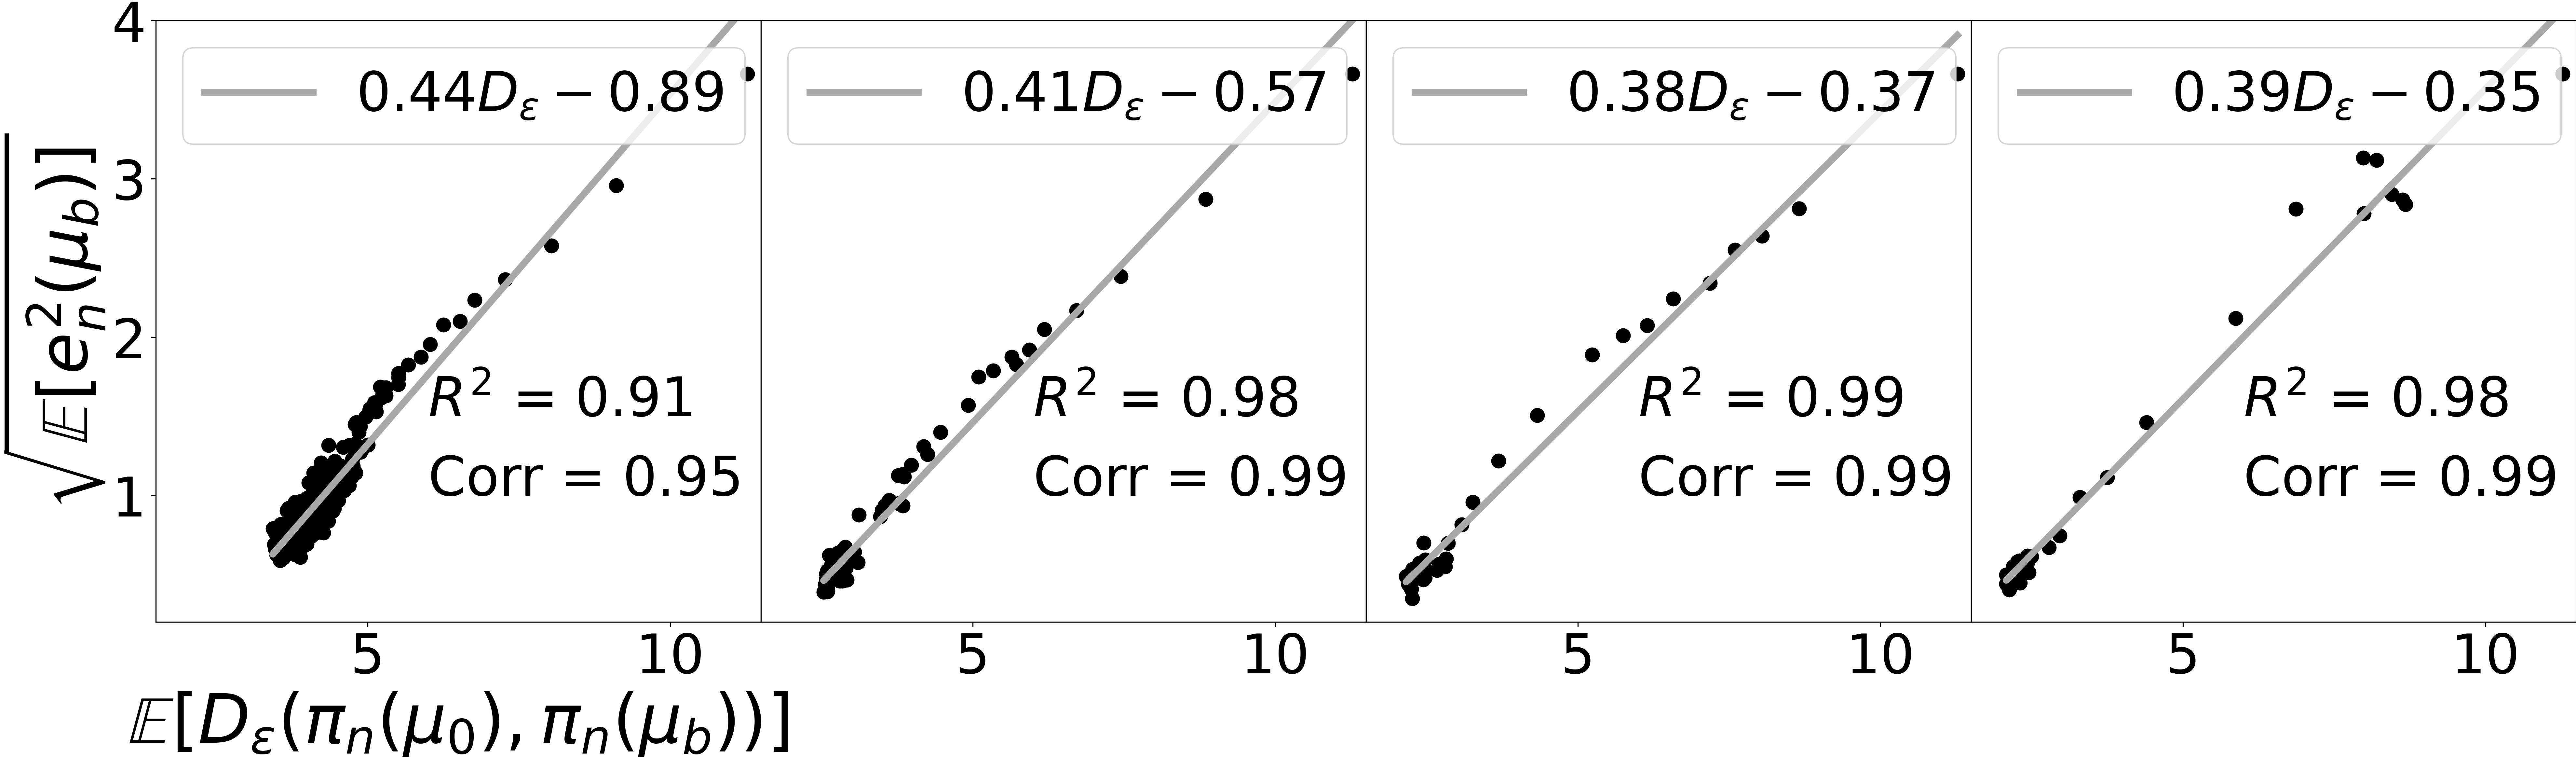
\includegraphics[width=0.48\columnwidth]{probing-nfs/plots/plots-bpf-effect of obs gap-dvl2_obs_gap_all.png} $\ \ $
    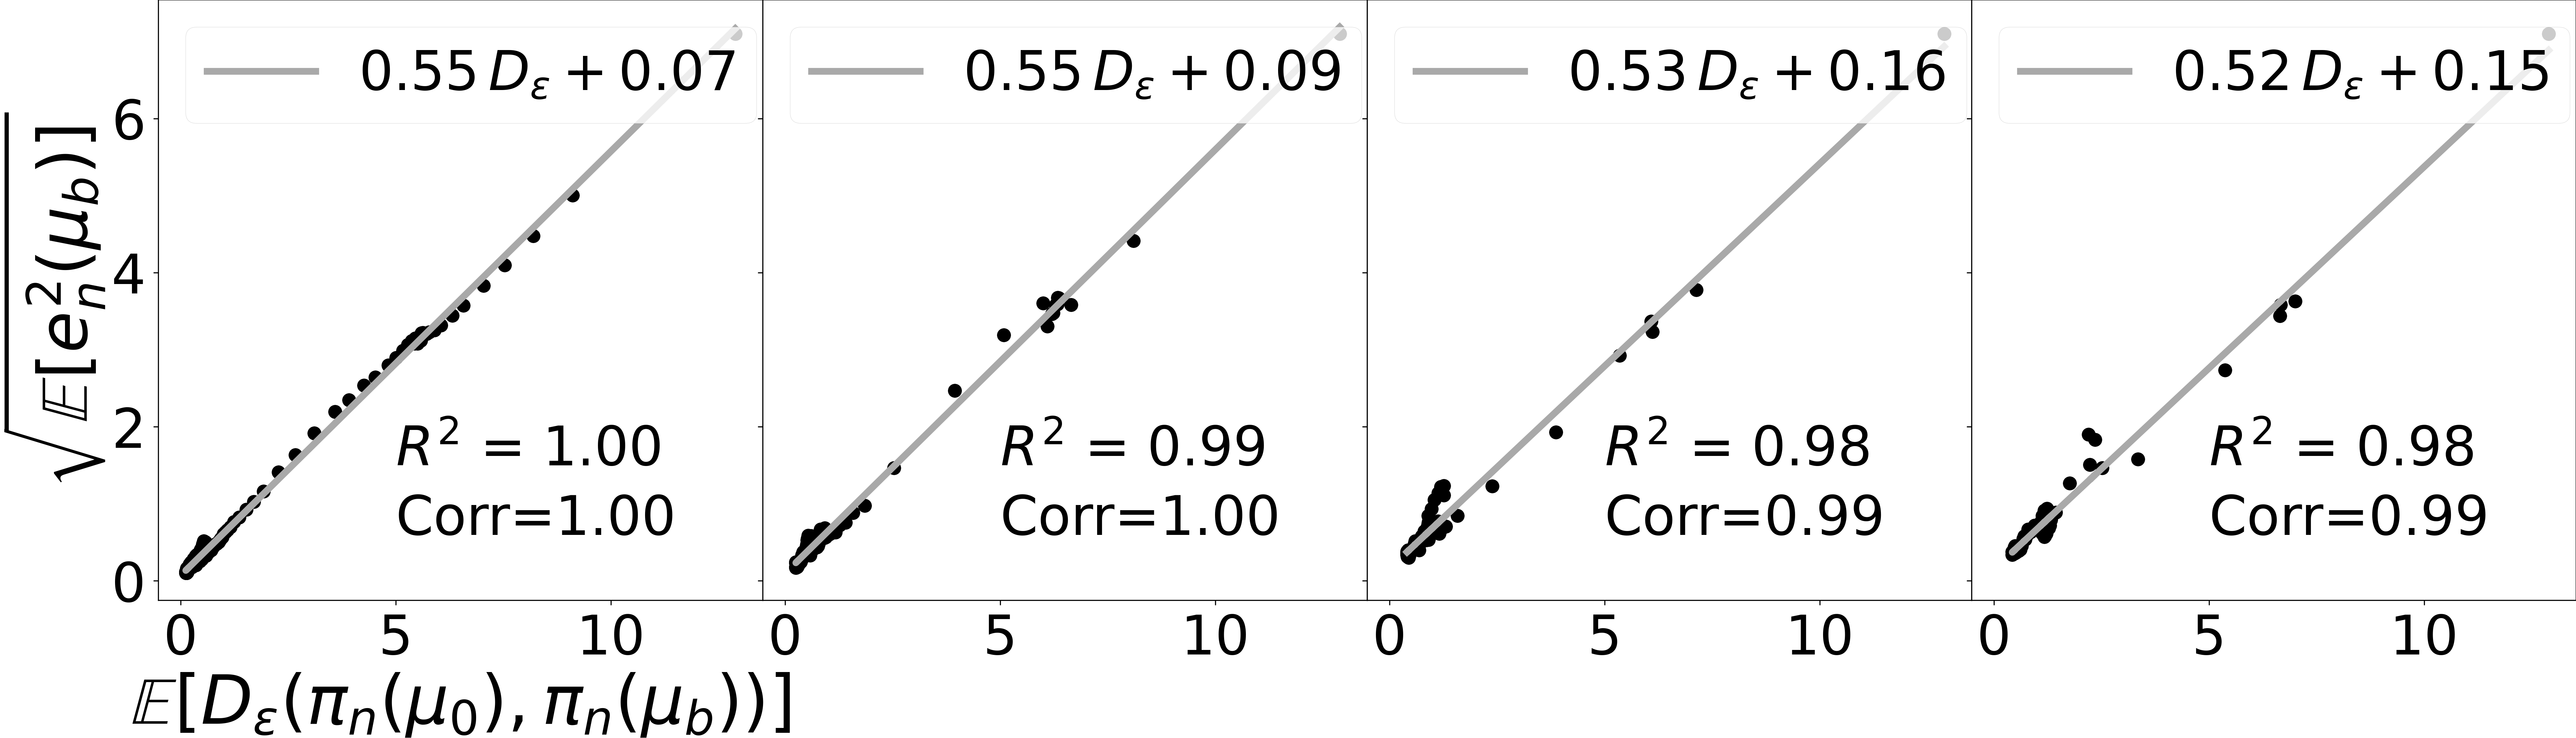
\includegraphics[width=0.48\textwidth]{probing-nfs/plots/plots-enkf-effect of ob gap-d_versus_l2_all.png}
\caption{The left and right panels show the results for PF and EnKF respectively with fixed observational error variance $\sigma^2 = 0.4$, and each column contains the results for different time between observations $g = 0.01, \, 0.03, \, 0.07, \, 0.09$.
Row 1: Mean $D_\varepsilon$ versus time. The dots represent 10 different realisations. The solid line is the exponential best-fit line for the mean $D_\varepsilon$ as in~\eqref{eq:fit--probing-nfs}.
Row 2: Mean scaled $l_2$ error from~\eqref{eq-error--probing-nfs} versus time for the two initial distributions.
Row 3: Mean uncertainty from~\eqref{eq-var--probing-nfs} versus time for the two initial distributions. The constant dotted line in rows 2 and 3 shows the observational error variance $\sigma^2$ for reference.
Row 4: RMSE versus mean $D_\varepsilon$. Pearson correlation coefficient between these two quantities is depicted alongside the goodness of fit for the best-fit line.}
\label{fig:bpf-enkf-fixed-ocov--probing-nfs}
\end{figure}



\begin{table}[t!]
\centering
\begin{tabular}{|c|c|c|c|c|c|} 
 \hline
\multicolumn{2}{|c|}{$g$} & $\bm{0.01}$ & $ \bm{0.03}$  & $\bm{0.07} $ & $\bm{0.09}$ \\ [0.5ex] 
\hline
\multirow{2}{*}{\text{a}} & \textbf{PF}& 5.367 $\pm$ 0.080 & 7.077 $\pm$ 0.055 & 8.672 $\pm$ 0.084 & 9.54 $\pm$ 0.40 \\\cline{2-6}
& \textbf{EnKF}& 9.28 $\pm$ 0.13 & 10.08 $\pm$ 0.27 & 11.11 $\pm$ 0.32 & 10.76 $\pm$ 0.37 \\
\hline
\multirow{2}{*}{$\lambda$}& \textbf{PF} & 10.73 $\pm$ 0.76 &  4.423 $\pm$ 0.058 & 2.203 $\pm$ 0.021 & 1.392 $\pm$ 0.052 \\ \cline{2-6}
& \textbf{EnKF} & 3.904 $\pm$ 0.085 &  3.56 $\pm$ 0.15 & 4.24 $\pm$ 0.21 & 2.95 $\pm$ 0.17 \\
\hline
\multirow{2}{*}{c} & \textbf{PF} & 4.03425 $\pm$ 0.00083 & 2.7524 $\pm$ 0.0018 & 2.1362 $\pm$ 0.0093 & 1.69 $\pm$ 0.14\\ \cline{2-6}
& \textbf{EnKF} & 0.258 $\pm$ 0.016 & 0.459 $\pm$ 0.036 & 0.711 $\pm$ 0.046 & 0.827 $\pm$ 0.064\\
\hline
\end{tabular}
\caption{Parameters of the best-fit for the mean $D_\varepsilon$ versus time as in~\eqref{eq:fit--probing-nfs} with associated confidence intervals for fixed observation covariance $\sigma^2 = 0.4$ and different observation gap $g$ shown in the top row.}
\label{table:fixcov--probing-nfs}
\end{table}

For PF, we see that the rate $\lambda$ decreases with increasing observation gap $g$ but for EnKF, the rates are not significantly affected by the change in $g$. The highest Lyapunov exponent for the model (with the chosen parameter value) is approximately $\lambda_{\text{max}} = 1.7$ whereas the exponential rate $\lambda$ for EnKF is seen to be in the range of $(3.0, 4.2)$, close to $2 \lambda_{\text{max}}$, indicating a possible close relation between the dynamics and the EnKF that could be explored further. The exponential rate for the PF does not seem to show such a relation.

Another difference between PF and EnKF may also be noted: with increasing observation gap, the stationary value $c$ for the PF decreases whereas it increases for the EnKF. Also, the stationary values $c$ of the $D_\varepsilon$ for EnKF are significantly lower compared to corresponding values for PF. These asymptotic values of $D_\varepsilon$ over time for both the filters can be explained by their mean posterior covariance using the following argument.

A characteristic of the numerical distance $D_\varepsilon$ is that for two different {\it i.i.d.}~samples drawn from the same probability distribution, $D_\varepsilon$ has a nonzero positive value. Statistically, $D_\varepsilon$ between two empirical measures approach this value at which they are essentially representing the same distribution and cannot be distinguished. For a fixed dimension $d$ and sample size $N$, this value increases with increasing covariance of the distribution \cite[Figure~1 and discussion therein]{mandal2021stability}.

The mean posterior covariance trace is directly proportional to the $s_n^2$. With increasing observation gap $g$, the mean uncertainty decreases for PF while it increases for EnKF. Hence the asymptotic value of $D_\varepsilon$ decreases with increasing observation gap for PF, while for the latter, it increases. We note that the previous paragraph explains the asymptotic value of $D_\varepsilon$, but the difference in the behaviour of the filter uncertainty $s_n$ for PF and EnKF as a function of observation gap needs to be explored further.

The scaled $l_2$ errors also reach an asymptotically constant value around the same time the corresponding filters stabilize in $D_\varepsilon$. The scatter plots for the RMSE against the $D_\varepsilon$ shows strong correlation between them. This suggests that we can use the RMSE over time as a good indicator for the time when the filter stabilizes. Note that the methods in this chapter give us a direct way to check whether a numerical filter is stable for a given dynamical and observational model, and the relation between the filter stability and the $l_2$ error or bias $e_n$ implies that a stable filter may be expected to be an accurate one.

We note that in the plots in the bottom row, the cluster at the bottom left corresponds to the time after which both RMSE and the $D_\varepsilon$ have reached their stationary values. Even for two different biased initial distributions for the filter, there is a finite transient growth after which the $D_\varepsilon$ falls exponentially \cite{mandal2021stability}. Although not shown here, the linear regime is still present in the scatter plot of the RMSE of either one of them versus the $D_\varepsilon$ in those cases. 

\subsection{Dependence on observation noise $\sigma$ }

We now discuss the results of numerical experiments with fixed observation gap $g = 0.05$, with varying observation covariance $\sigma^2 = 0.2, 0.4, 0.8, 1.6$. In figure \ref{fig:bpf-enkf-fixed-ogap--probing-nfs}, we again note the exponential decrease of the distance $D_\varepsilon$ over time until it reaches a stationary value $c$. The parameter values obtained for the best-fit for different observation covariance are shown in table \ref{table:fixgap--probing-nfs}.




\begin{figure}[t!]
\centering
Particle filter $\qquad \qquad \qquad \qquad \qquad \qquad \qquad \qquad $ EnKF\\
    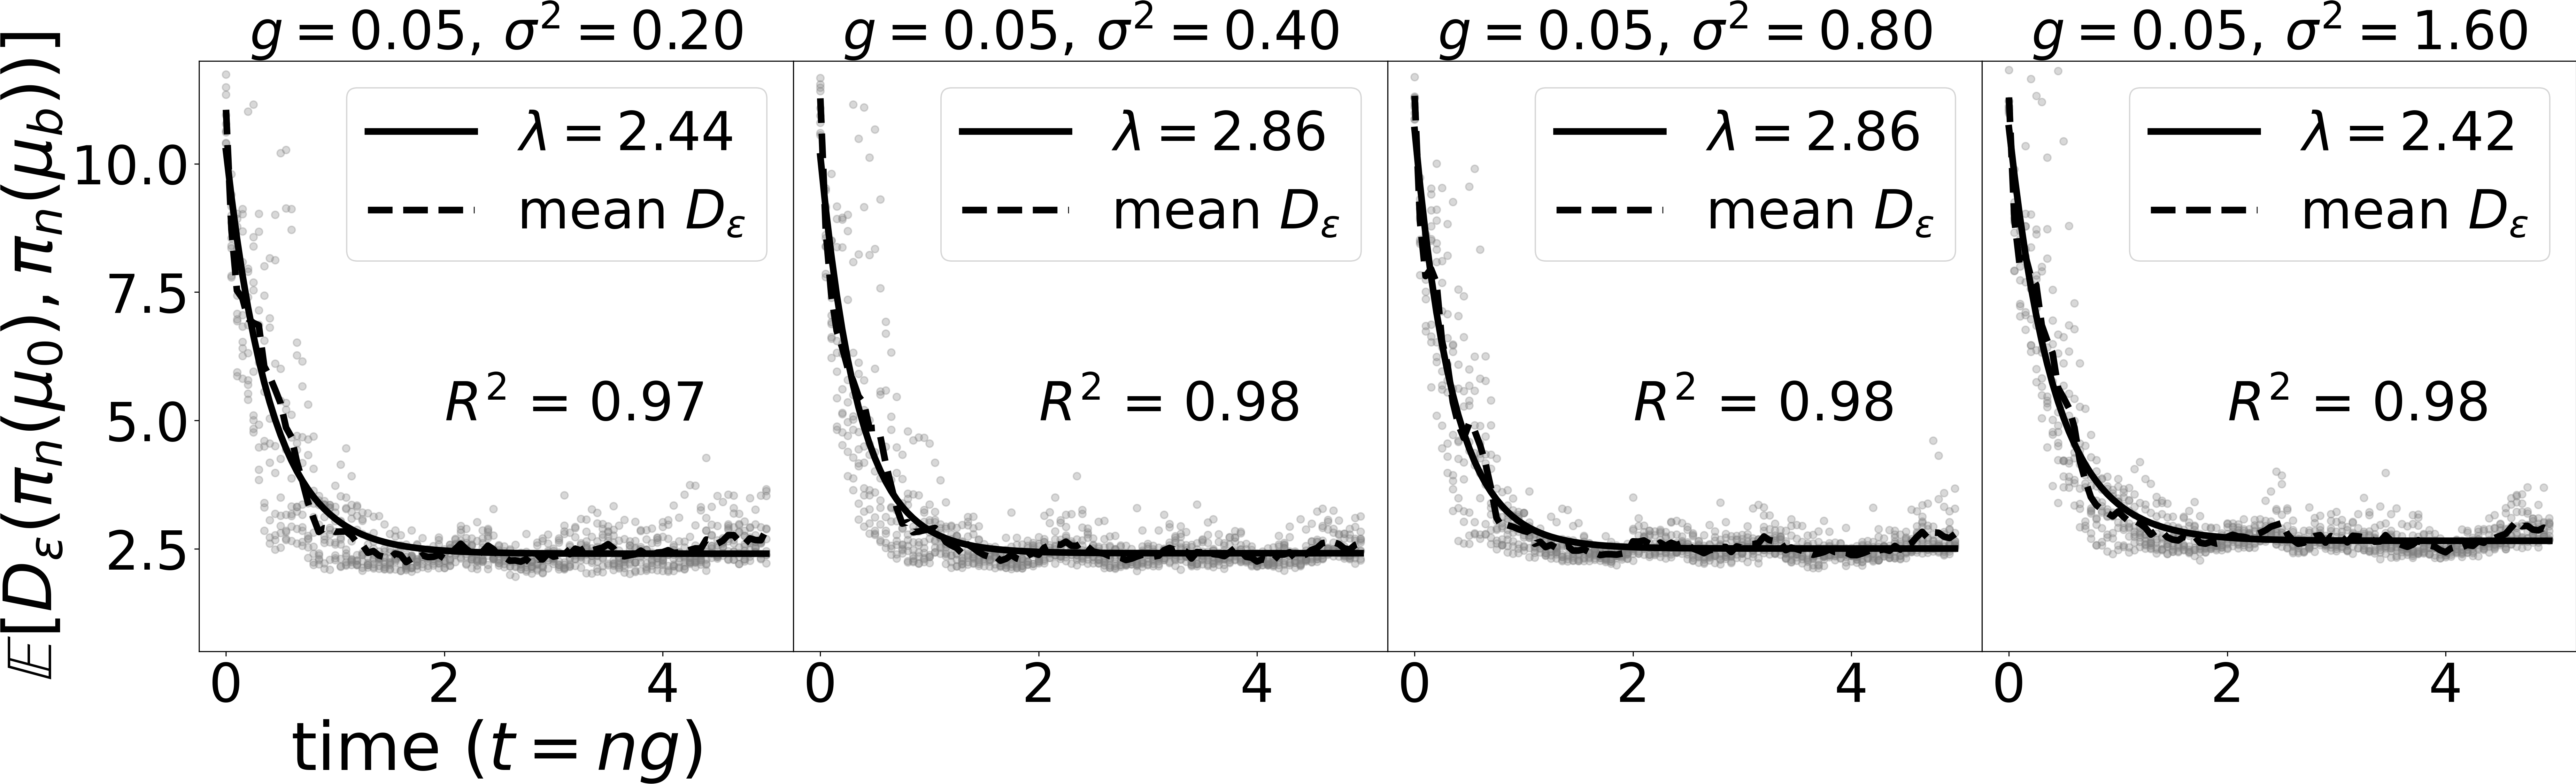
\includegraphics[width=0.48\textwidth]{probing-nfs/plots/plots-bpf-effect of obs cov-rate_obs_cov_all.png} $\ \ $
    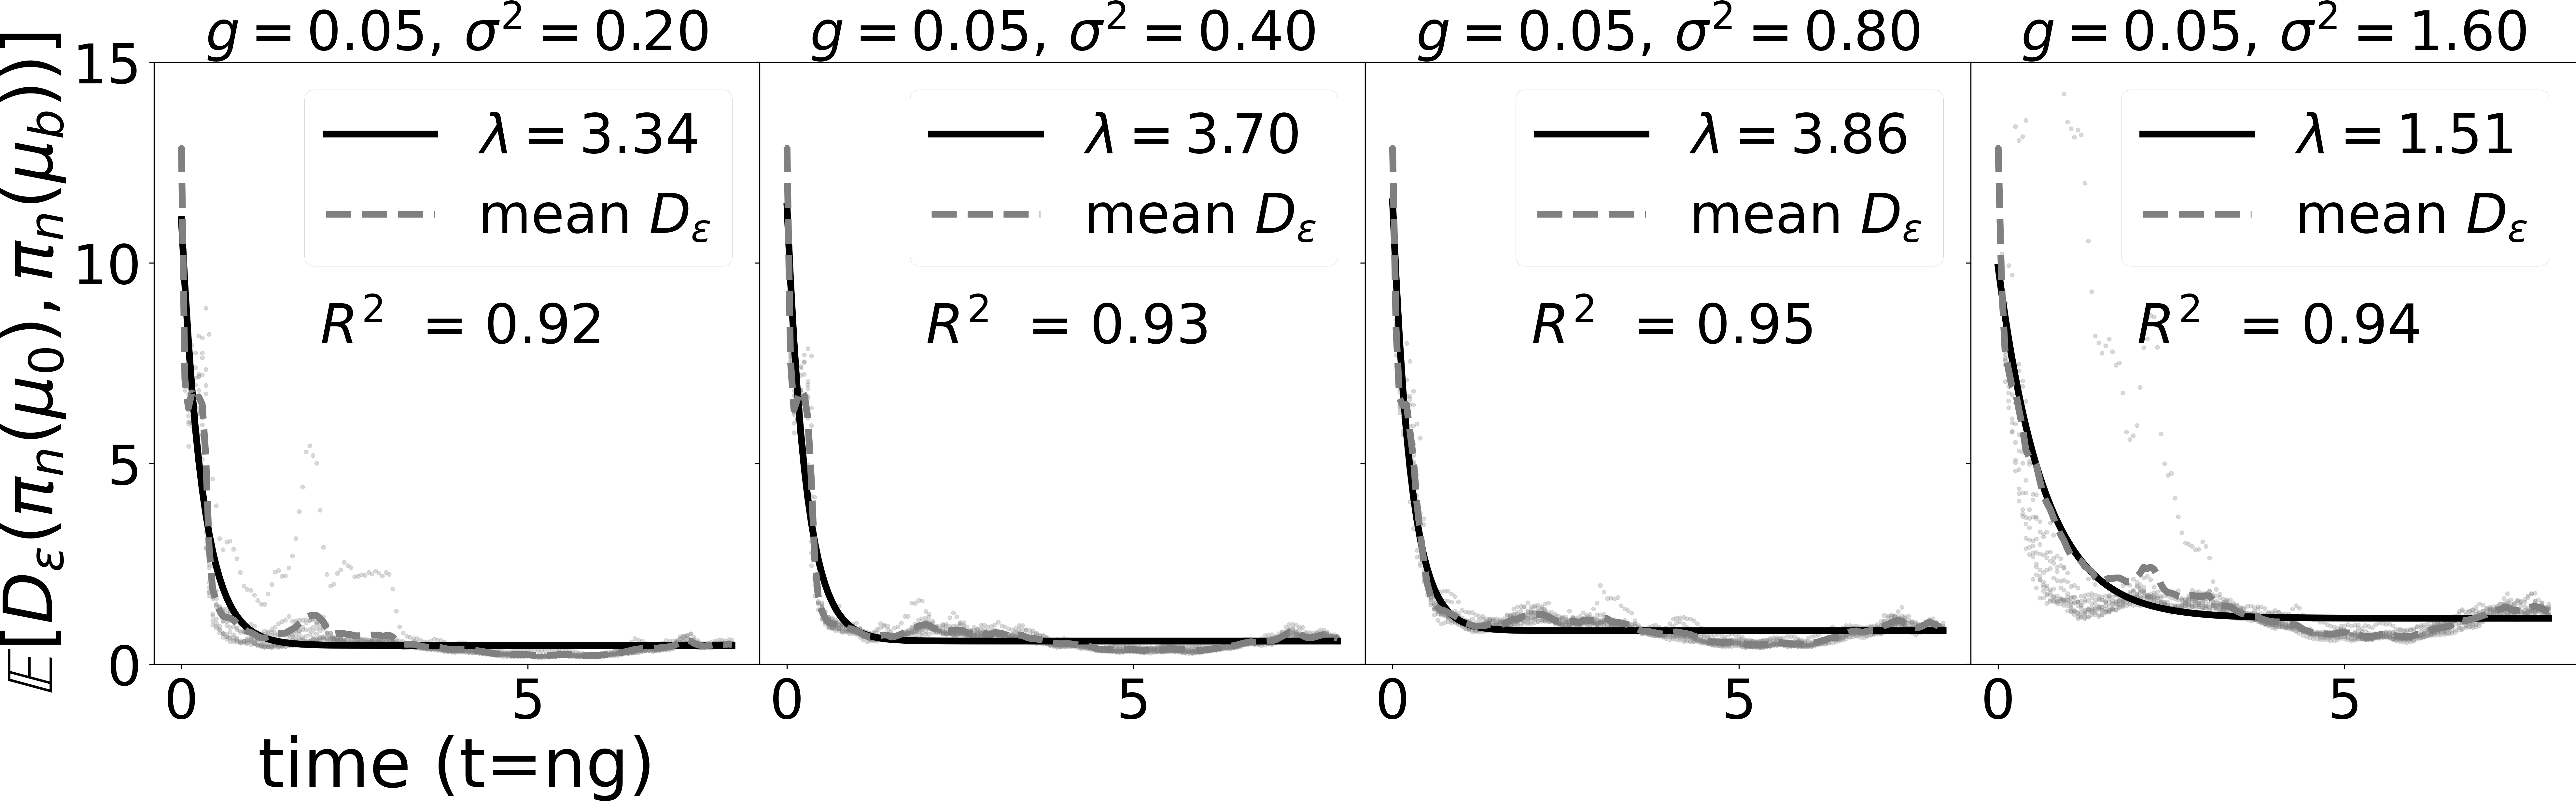
\includegraphics[width=0.48\textwidth]{probing-nfs/plots/plots-enkf-effect of ob cov-rate_all.png}\\
   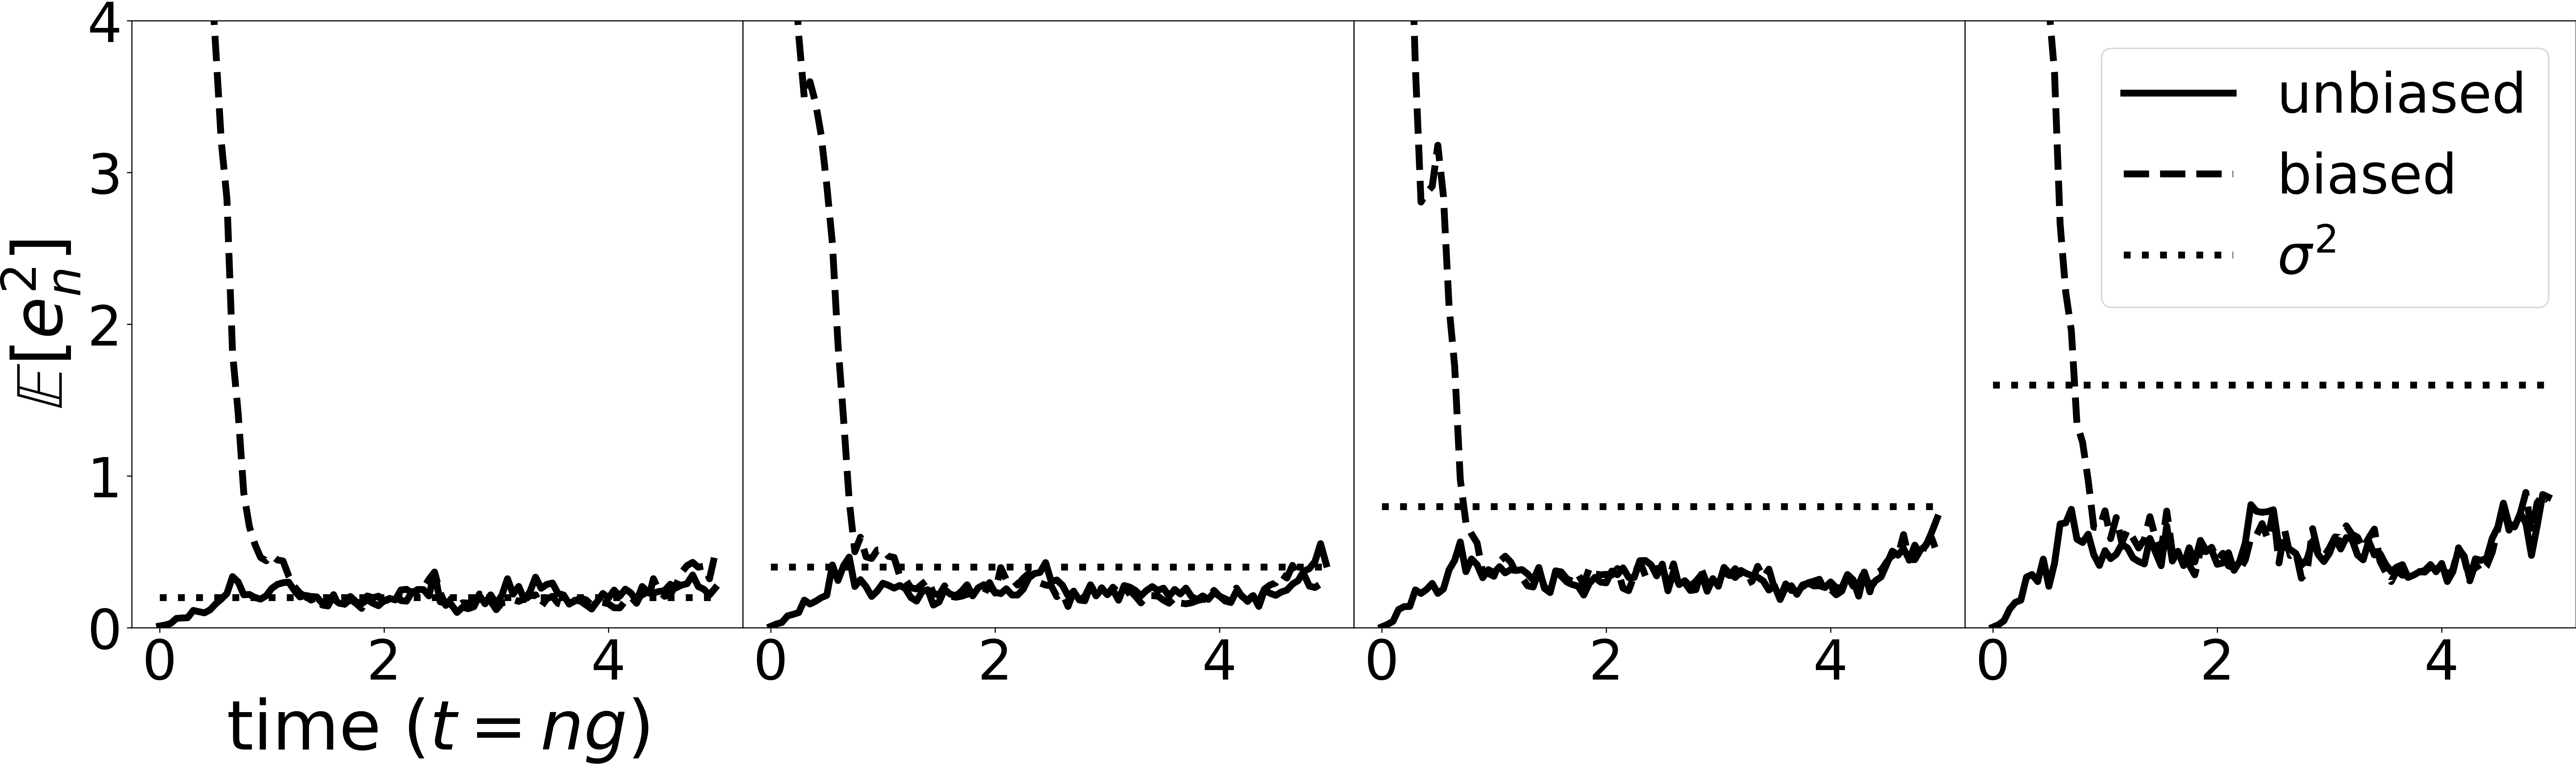
\includegraphics[width=0.48\columnwidth]{probing-nfs/plots/plots-bpf-effect of obs cov-l2_obs_cov_all.png} $\ \ $
    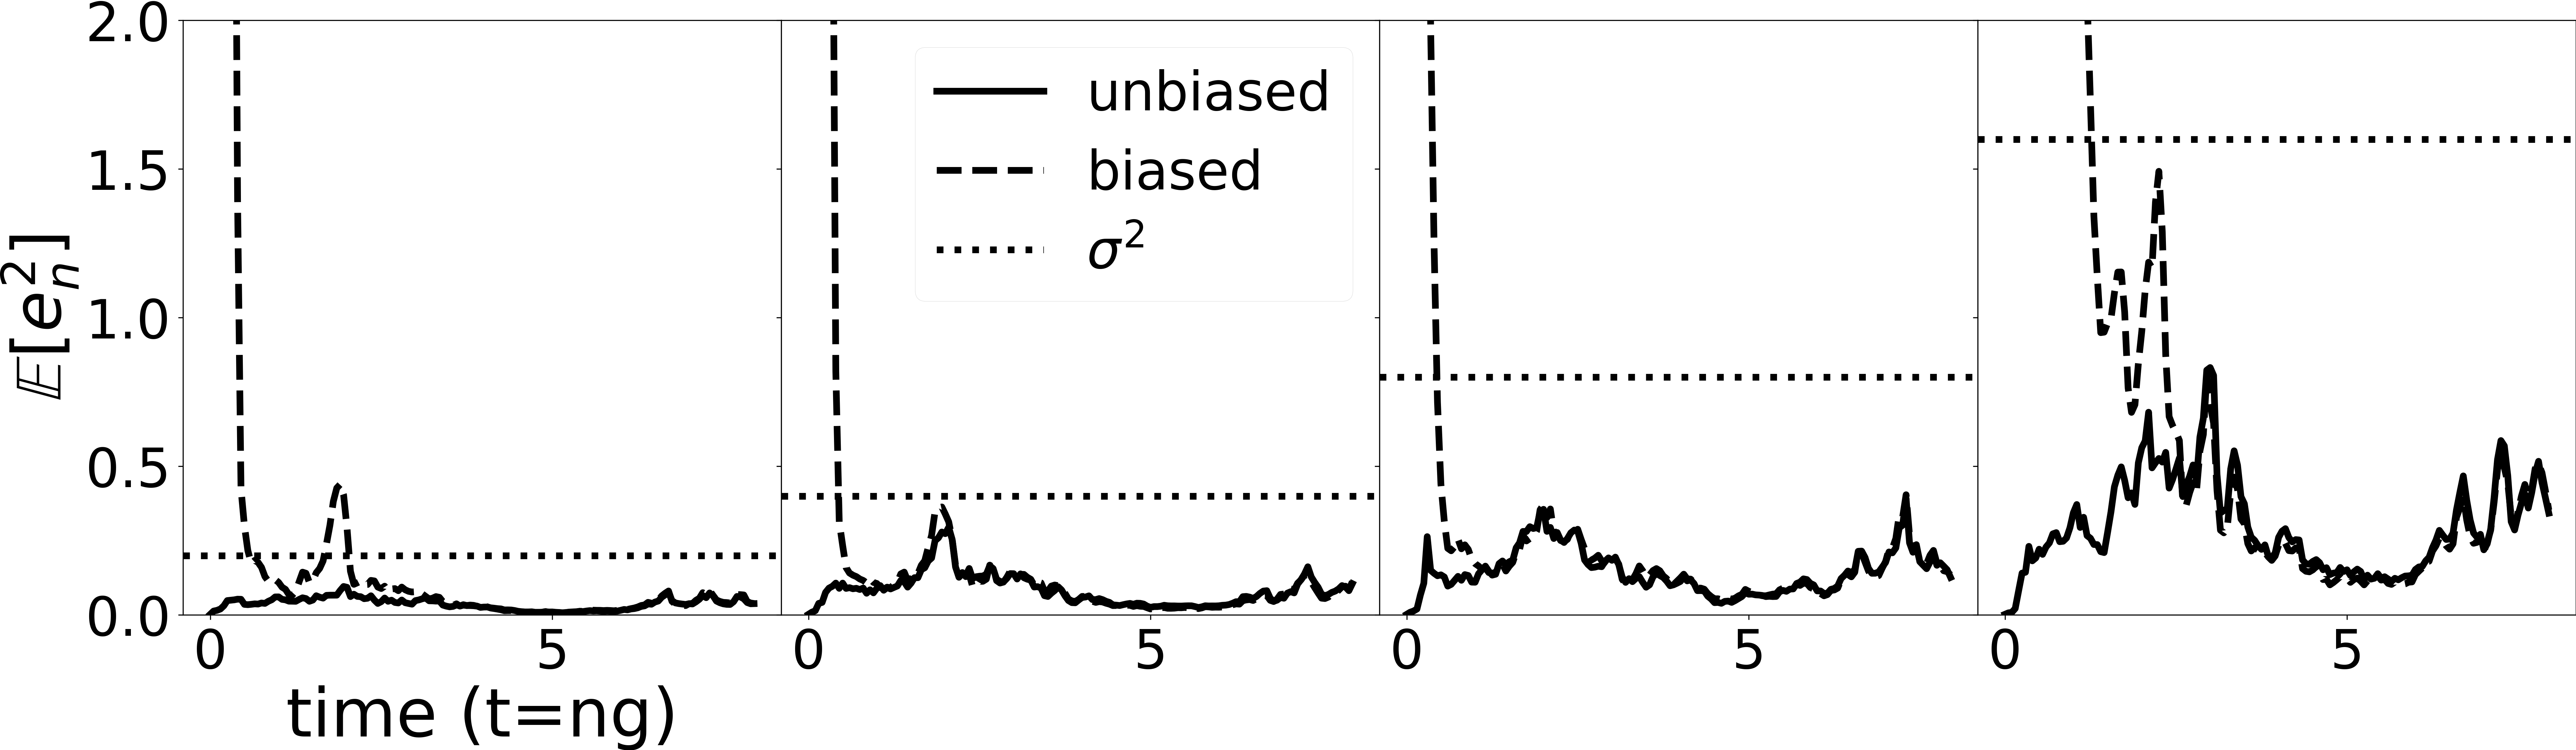
\includegraphics[width=0.48\textwidth]{probing-nfs/plots/plots-enkf-effect of ob cov-mean_l2error_all.png}\\
   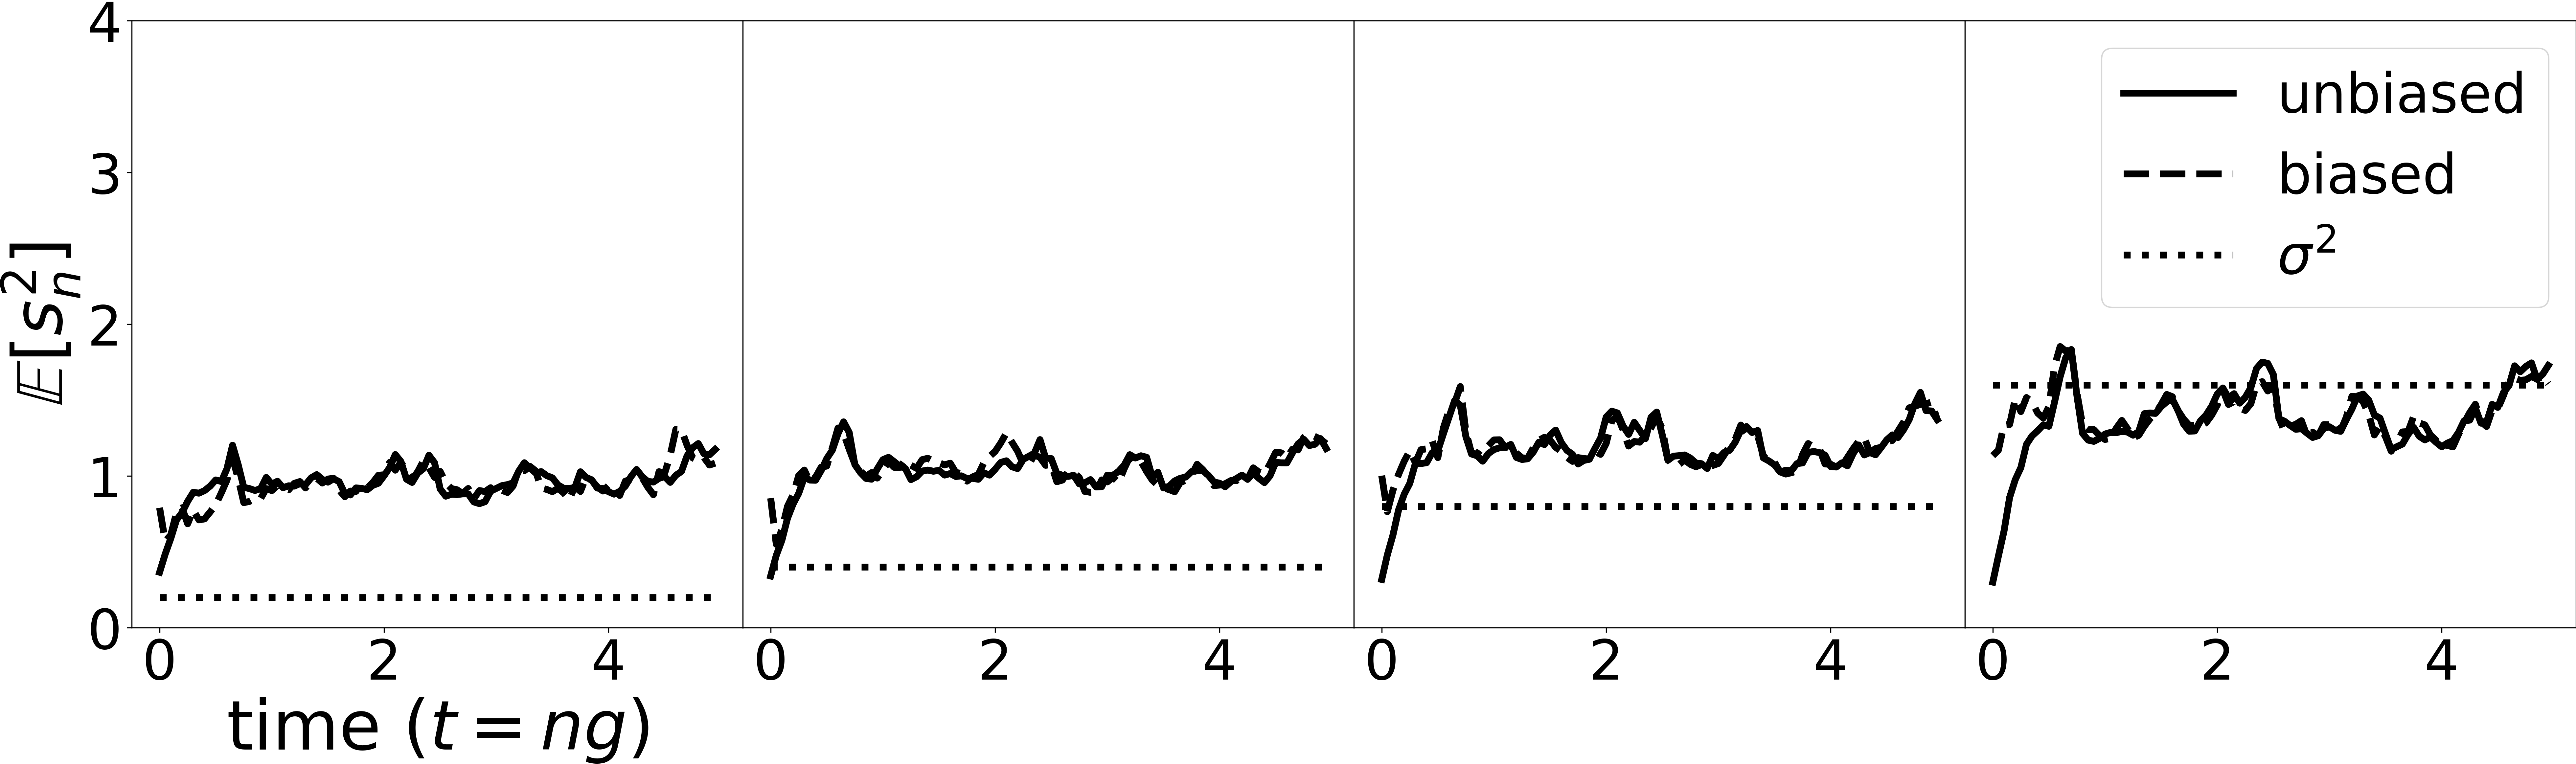
\includegraphics[width=0.48\columnwidth]{probing-nfs/plots/plots-bpf-effect of obs cov-trace_obs_cov_all.png} $\ \ $
    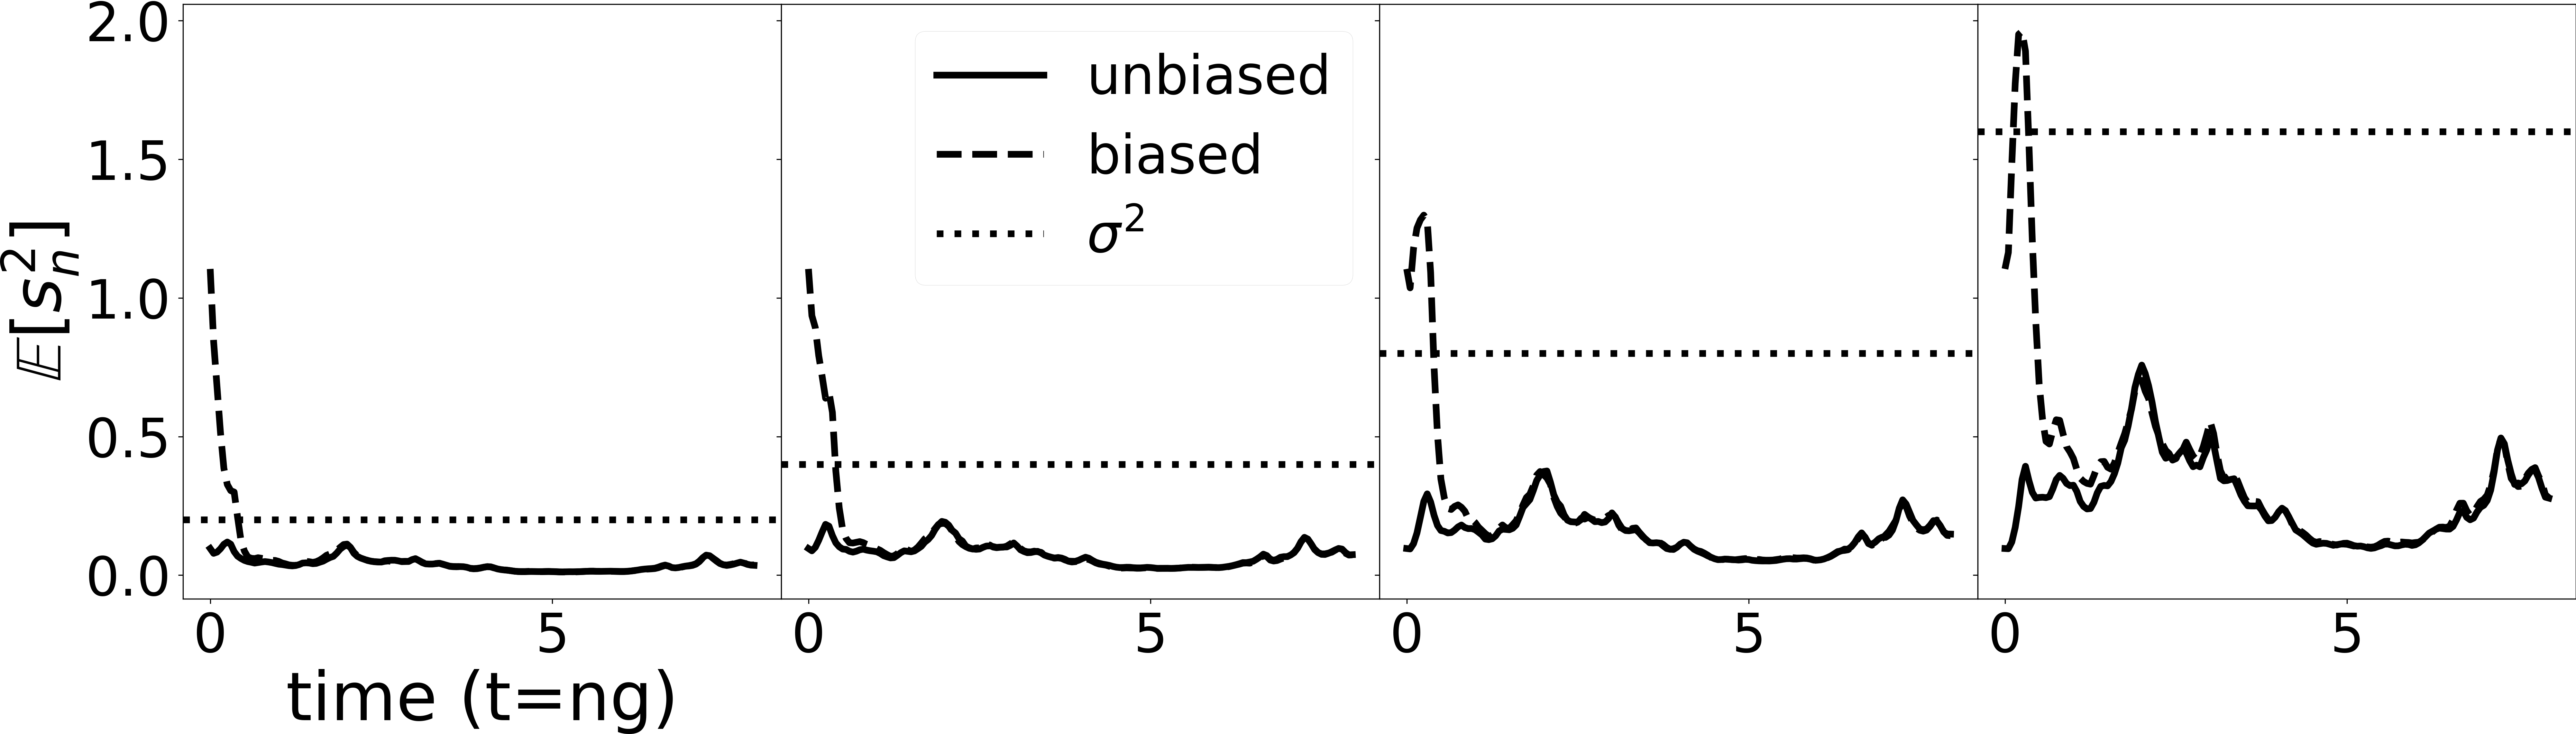
\includegraphics[width=0.48\textwidth]{probing-nfs/plots/plots-enkf-effect of ob cov-mean_trace_all.png}\\
   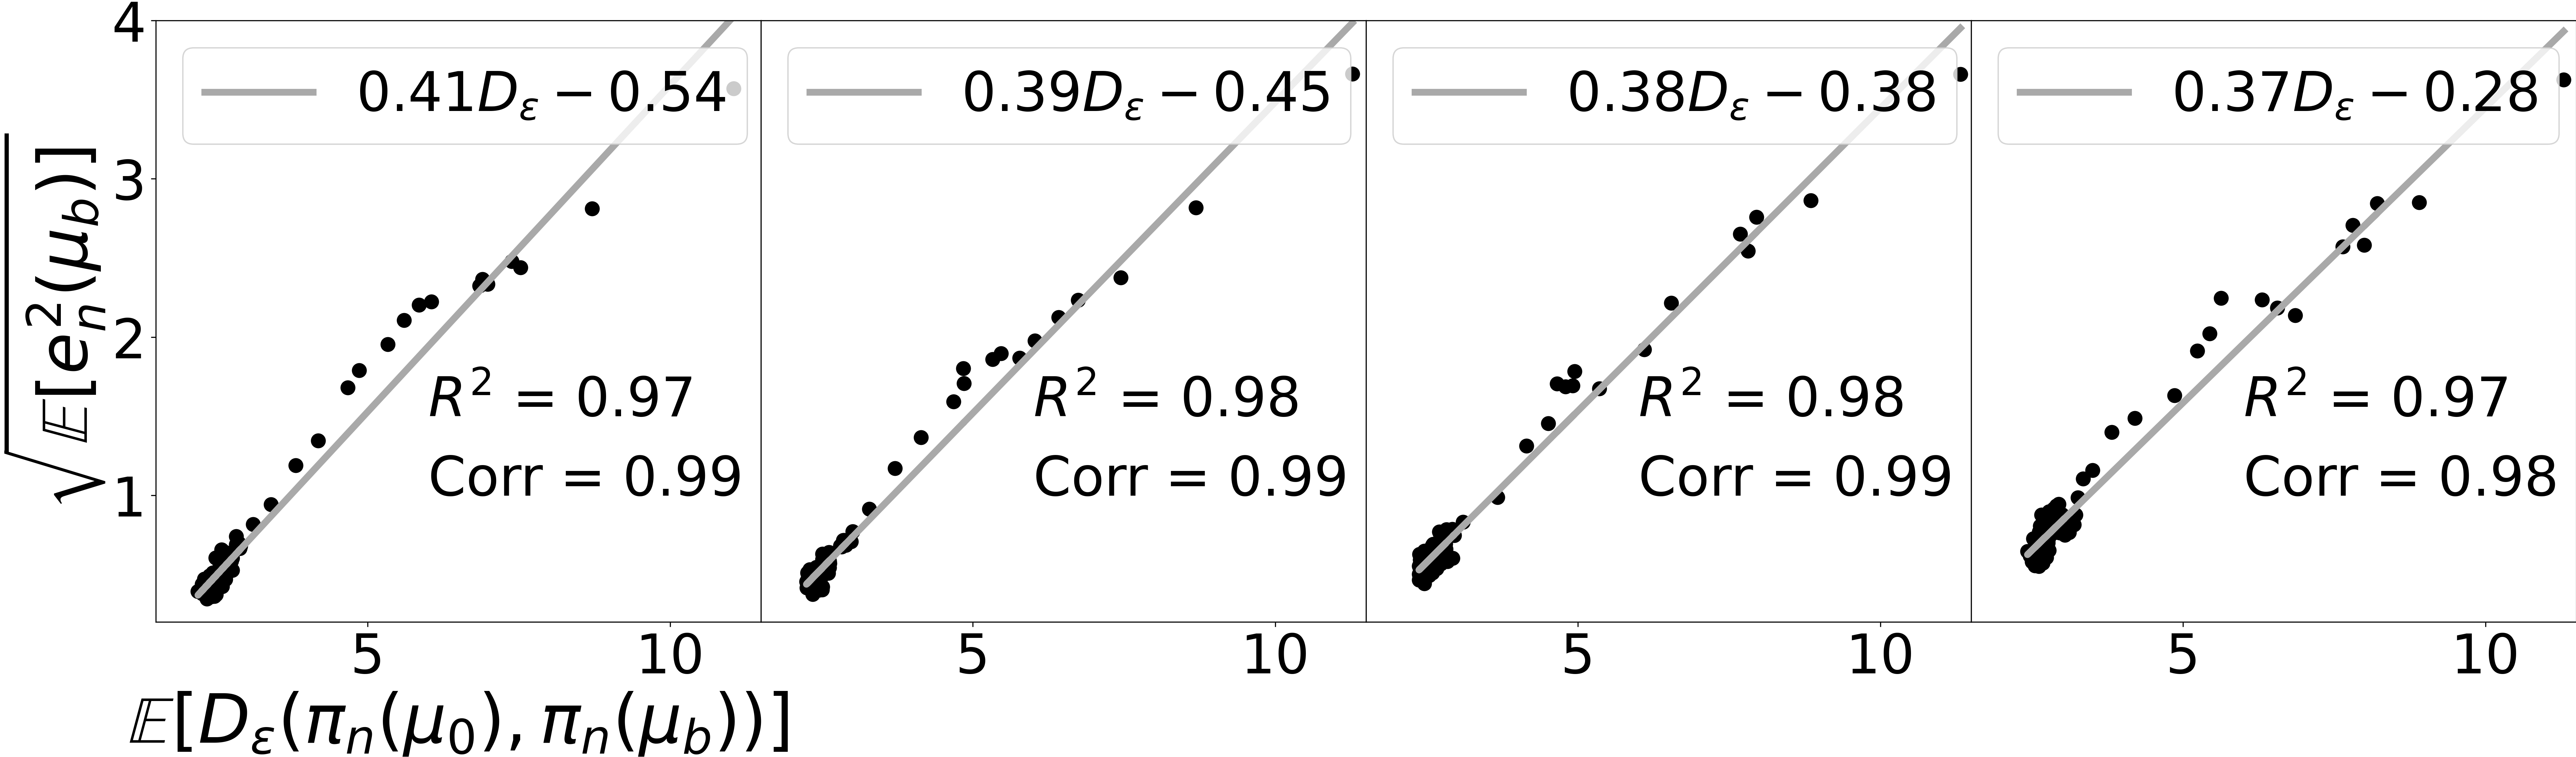
\includegraphics[width=0.48\columnwidth]{probing-nfs/plots/plots-bpf-effect of obs cov-dvl2_obs_cov_all.png} $\ \ $
    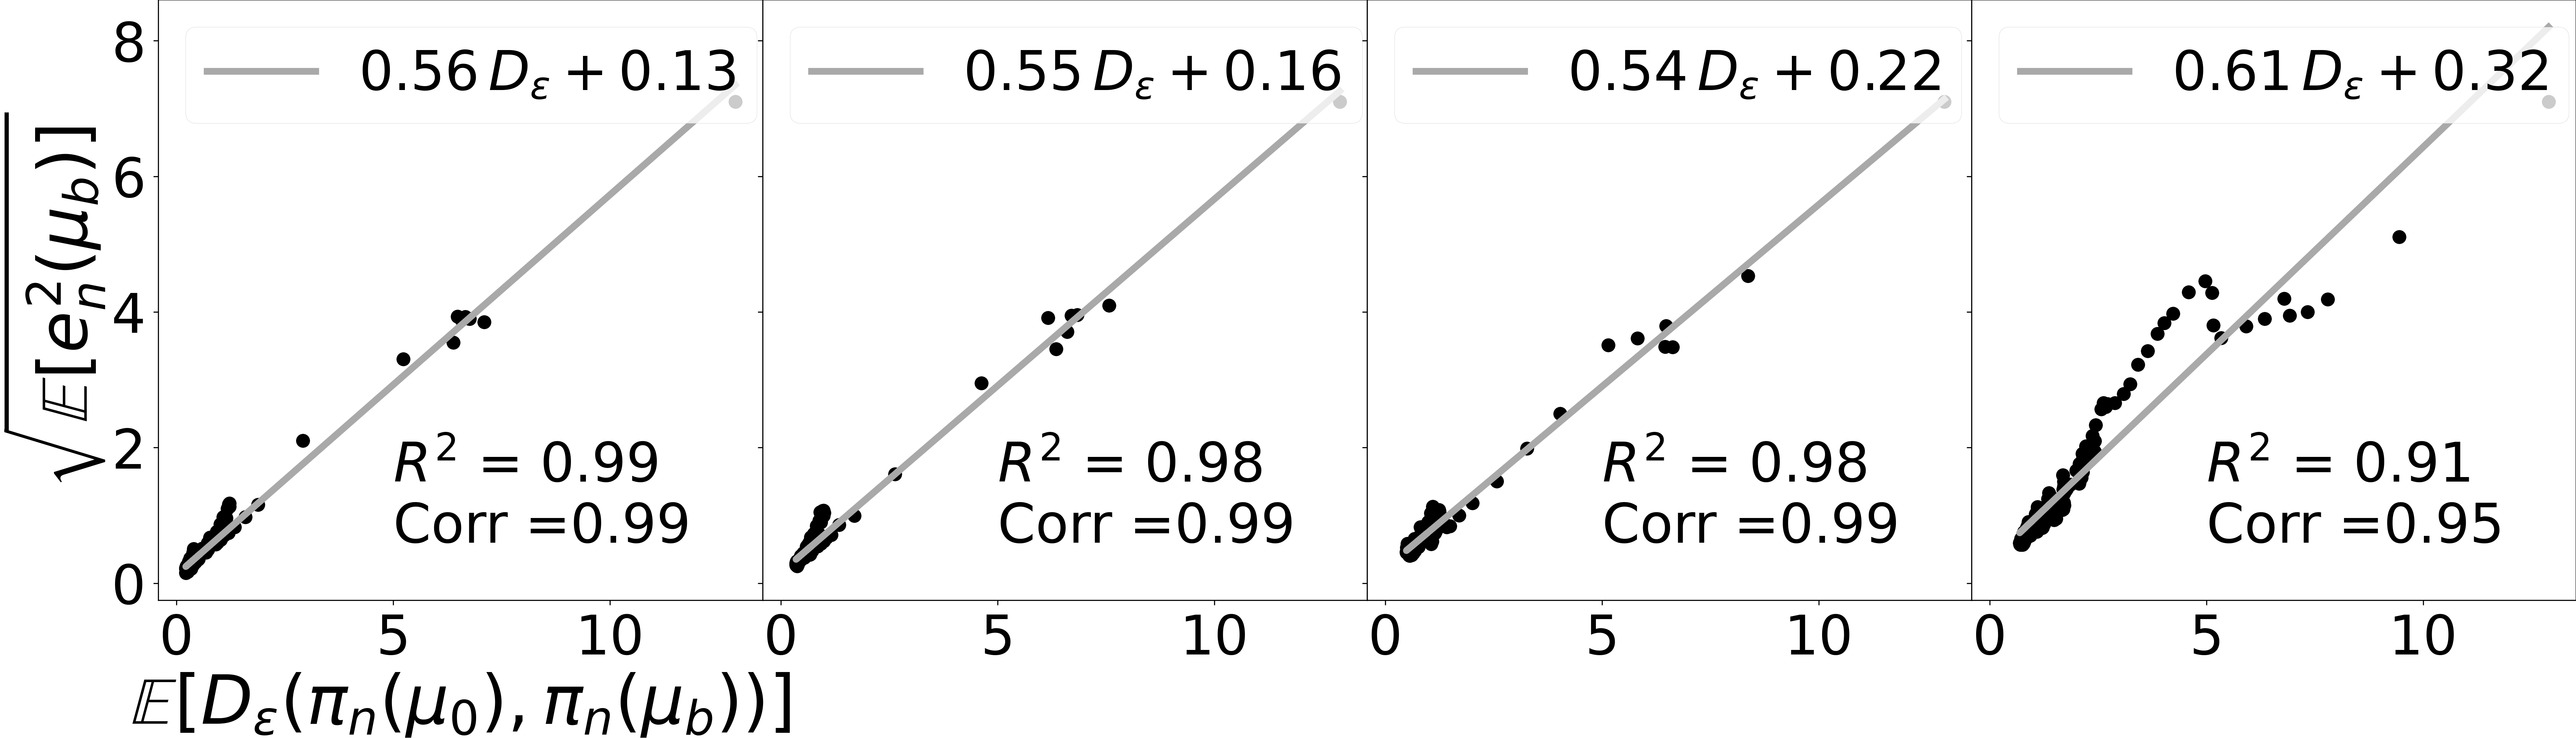
\includegraphics[width=0.48\textwidth]{probing-nfs/plots/plots-enkf-effect of ob cov-d_versus_l2_all.png}
\caption{Same as in figure~\ref{fig:bpf-enkf-fixed-ocov--probing-nfs} with the left and right panels showing the results for PF and EnKF respectively, but with fixed time between observations $g = 0.05$, and each column containing the results for different observational error variances of $\sigma^2 = 0.2, \, 0.4, \, 0.8, \, 1.6$.}
\label{fig:bpf-enkf-fixed-ogap--probing-nfs}
\end{figure}


\begin{table}[t!]
\centering
\begin{tabular}{|c|c|c|c|c|c|} 
 \hline
 
\multicolumn{2}{|c|}{$\sigma^2$} & $\bm{0.2}$ & $ \bm{0.4}$  & $\bm{0.8} $ & $\bm{1.6}$ \\ [0.5ex] 
\hline
\multirow{2}{*}{\text{a}} & \textbf{PF}& 7.842 $\pm$ 0.058 & 7.730 $\pm$ 0.046 & 8.153 $\pm$ 0.044 & 8.038 $\pm$ 0.048 \\\cline{2-6}
& \textbf{EnKF}& 10.61 $\pm$ 0.32 & 10.84 $\pm$ 0.30 & 10.69 $\pm$ 0.23 & 8.75 $\pm$ 0.22 \\
\hline
\multirow{2}{*}{$\lambda$}& \textbf{PF} & 2.442 $\pm$ 0.016 &  2.858 $\pm$ 0.017 & 2.859 $\pm$ 0.015 & 2.416 $\pm$ 0.012 \\ \cline{2-6}
& \textbf{EnKF} & 3.34 $\pm$ 0.16 &  3.70 $\pm$ 0.16 & 3.86 $\pm$ 0.14 & 1.507 $\pm$ 0.062 \\
\hline
\multirow{2}{*}{c} & \textbf{PF} & 2.4050 $\pm$ 0.0022 & 2.4144 $\pm$ 0.0015 & 2.5051 $\pm$ 0.0014 & 2.6554 $\pm$ 0.0019\\ \cline{2-6}
& \textbf{EnKF} & 0.470 $\pm$ 0.039 & 0.579 $\pm$ 0.035 & 0.838 $\pm$ 0.027 & 1.148 $\pm$ 0.041\\
\hline
\end{tabular}
\caption{Parameters of the best-fit for the mean $D_\varepsilon$ versus time as in~\eqref{eq:fit--probing-nfs} with associated confidence intervals for fixed observation gap $g = 0.05$ and different observational error covariance $\sigma^2$ shown in the top row.}
\label{table:fixgap--probing-nfs}
\end{table}

In contrast with the case of varying observational gap, the exponential rates for the PF stability are not affected by the change in observational uncertainty. While the rates for EnKF are again close to twice the Lyapunov exponent, the rates for PF are smaller.

The scaled $l_2$ error and the $D_\varepsilon$ achieve their stationary value around the same time as in the former case of fixed observation. As expected, this asymptotic value $c$ as well as the asymptotic values of the uncertainty $s_n$ and the bias $e_n$ all increase with increasing $\sigma^2$ for both PF and EnKF.  

We also see near perfect correlation in the scatter plots for the RMSE versus mean $D_\varepsilon$ as for both PF and EnKF, we get pearson correlation coefficient very close to 1. We remark that in our numerical experiments, either with varying observational time gap or with varying observational covariance, we did not notice any relation between stability and posterior uncertainty or precision, i.e., there did not seem to be any relation between $D_\varepsilon$ and $s_n$.

